\fancyfoot[C]{Kronberger}

%% Human-Computer Interaction System %%%%%%%%%%%%%%%%%%%%%%%

\chapter{Human-Computer Interaction System}

\section{Übersicht}

Das Human-Computer Interaction System ist, wie der Name schon sagt, die Komponente, welche als Schnittstelle zwischen dem Nutzer und dem gesamten elektrischen System dient. Durch es sollte die fehlerfreie Nutzung der Funktionen des Motorrades gewährleistet sein. Ebenso sollte es wichtige Fahrdaten und andere Informationen speichern und dem User anzeigen können.\\
Wichtig ist das System, trotz der großen Komplexität, so intuitiv und nutzerfreundlich wie möglich zu gestalten.

\subsection{Grundfunktionen des Systems}

Die geplanten Funktionen des HCIS \footnote{Abkurzümg: Human-Computer Interaction System} lassen sich grob in vier Grundfunktionen einteilen.

\begin{itemize}

	\item \textbf{Steuerung der Peripherie} \medskip\\
	Die Schalter und Buttons am Lenker, welche zuvor über den Kabelbaum die Leuchten, Blinker und die Hupe gesteuert haben, werden nun über die General-purpose input/output (GPIO) des Raspberry Pi Mikrocomputers gesteuert.

	\item \textbf{Graphische Benutzeroberfläche}\medskip\\
Dient der Anzeige wichtiger Fahr- und Ladedaten, welche entweder in Echtzeit oder über die Datenbankschnittstelle abgerufen und graphisch angezeigt werden können.

	\item \textbf{Kommunikation mit den Steuereinheiten des Motorrades} \medskip\\
	Über CAN-Bus werden Daten von dem Batterie Management Systems (BMS) und der Curtis Motorsteuerung empfangen und an die Benutzeroberfläche zur Anzeige und an die Datenbankschnittstelle zur Langzeitsicherung der Fahrdaten weiter gegeben.

	\item \textbf{Speichern der relevanten Fahrdaten über die Datenbankschnittstelle} \medskip\\
Die über den CAN-Bus empfangenen Daten werden sofort an die Datenbankschnittstelle (Handler) weitergegeben um die Daten für Datenauswertung und Testberichte zu speichern. Ebenso bezieht das Diagnosesystem der Benutzeroberfläche die Daten über diese Schnittstelle.

\end{itemize}

\newpage

\subsection{Steuereinheit}

Als Basis zur Auswahl der Steuereinheit wurden die zuvor erläuterten Grundfunktionen herangezogen genommen. Die Ausgewählte Steuereinheit sollte diese erfüllen können und ebenso Potential zur Erweiterung der Funktionen bieten. Genauso wichtig war das eine große Flexibilität und Individualität erreicht werden kann, um nicht in der Umsetzung unserer Ideen eingeschränkt zu sein. Zur Auswahl standen verschiedene Speicherprogrammierbare Steuerungen und Mikrocomputer, doch letzten Endes überzeugte der Mikrocomputer Raspberry Pi.

\begin{figure}[H]
	\begin{center}
		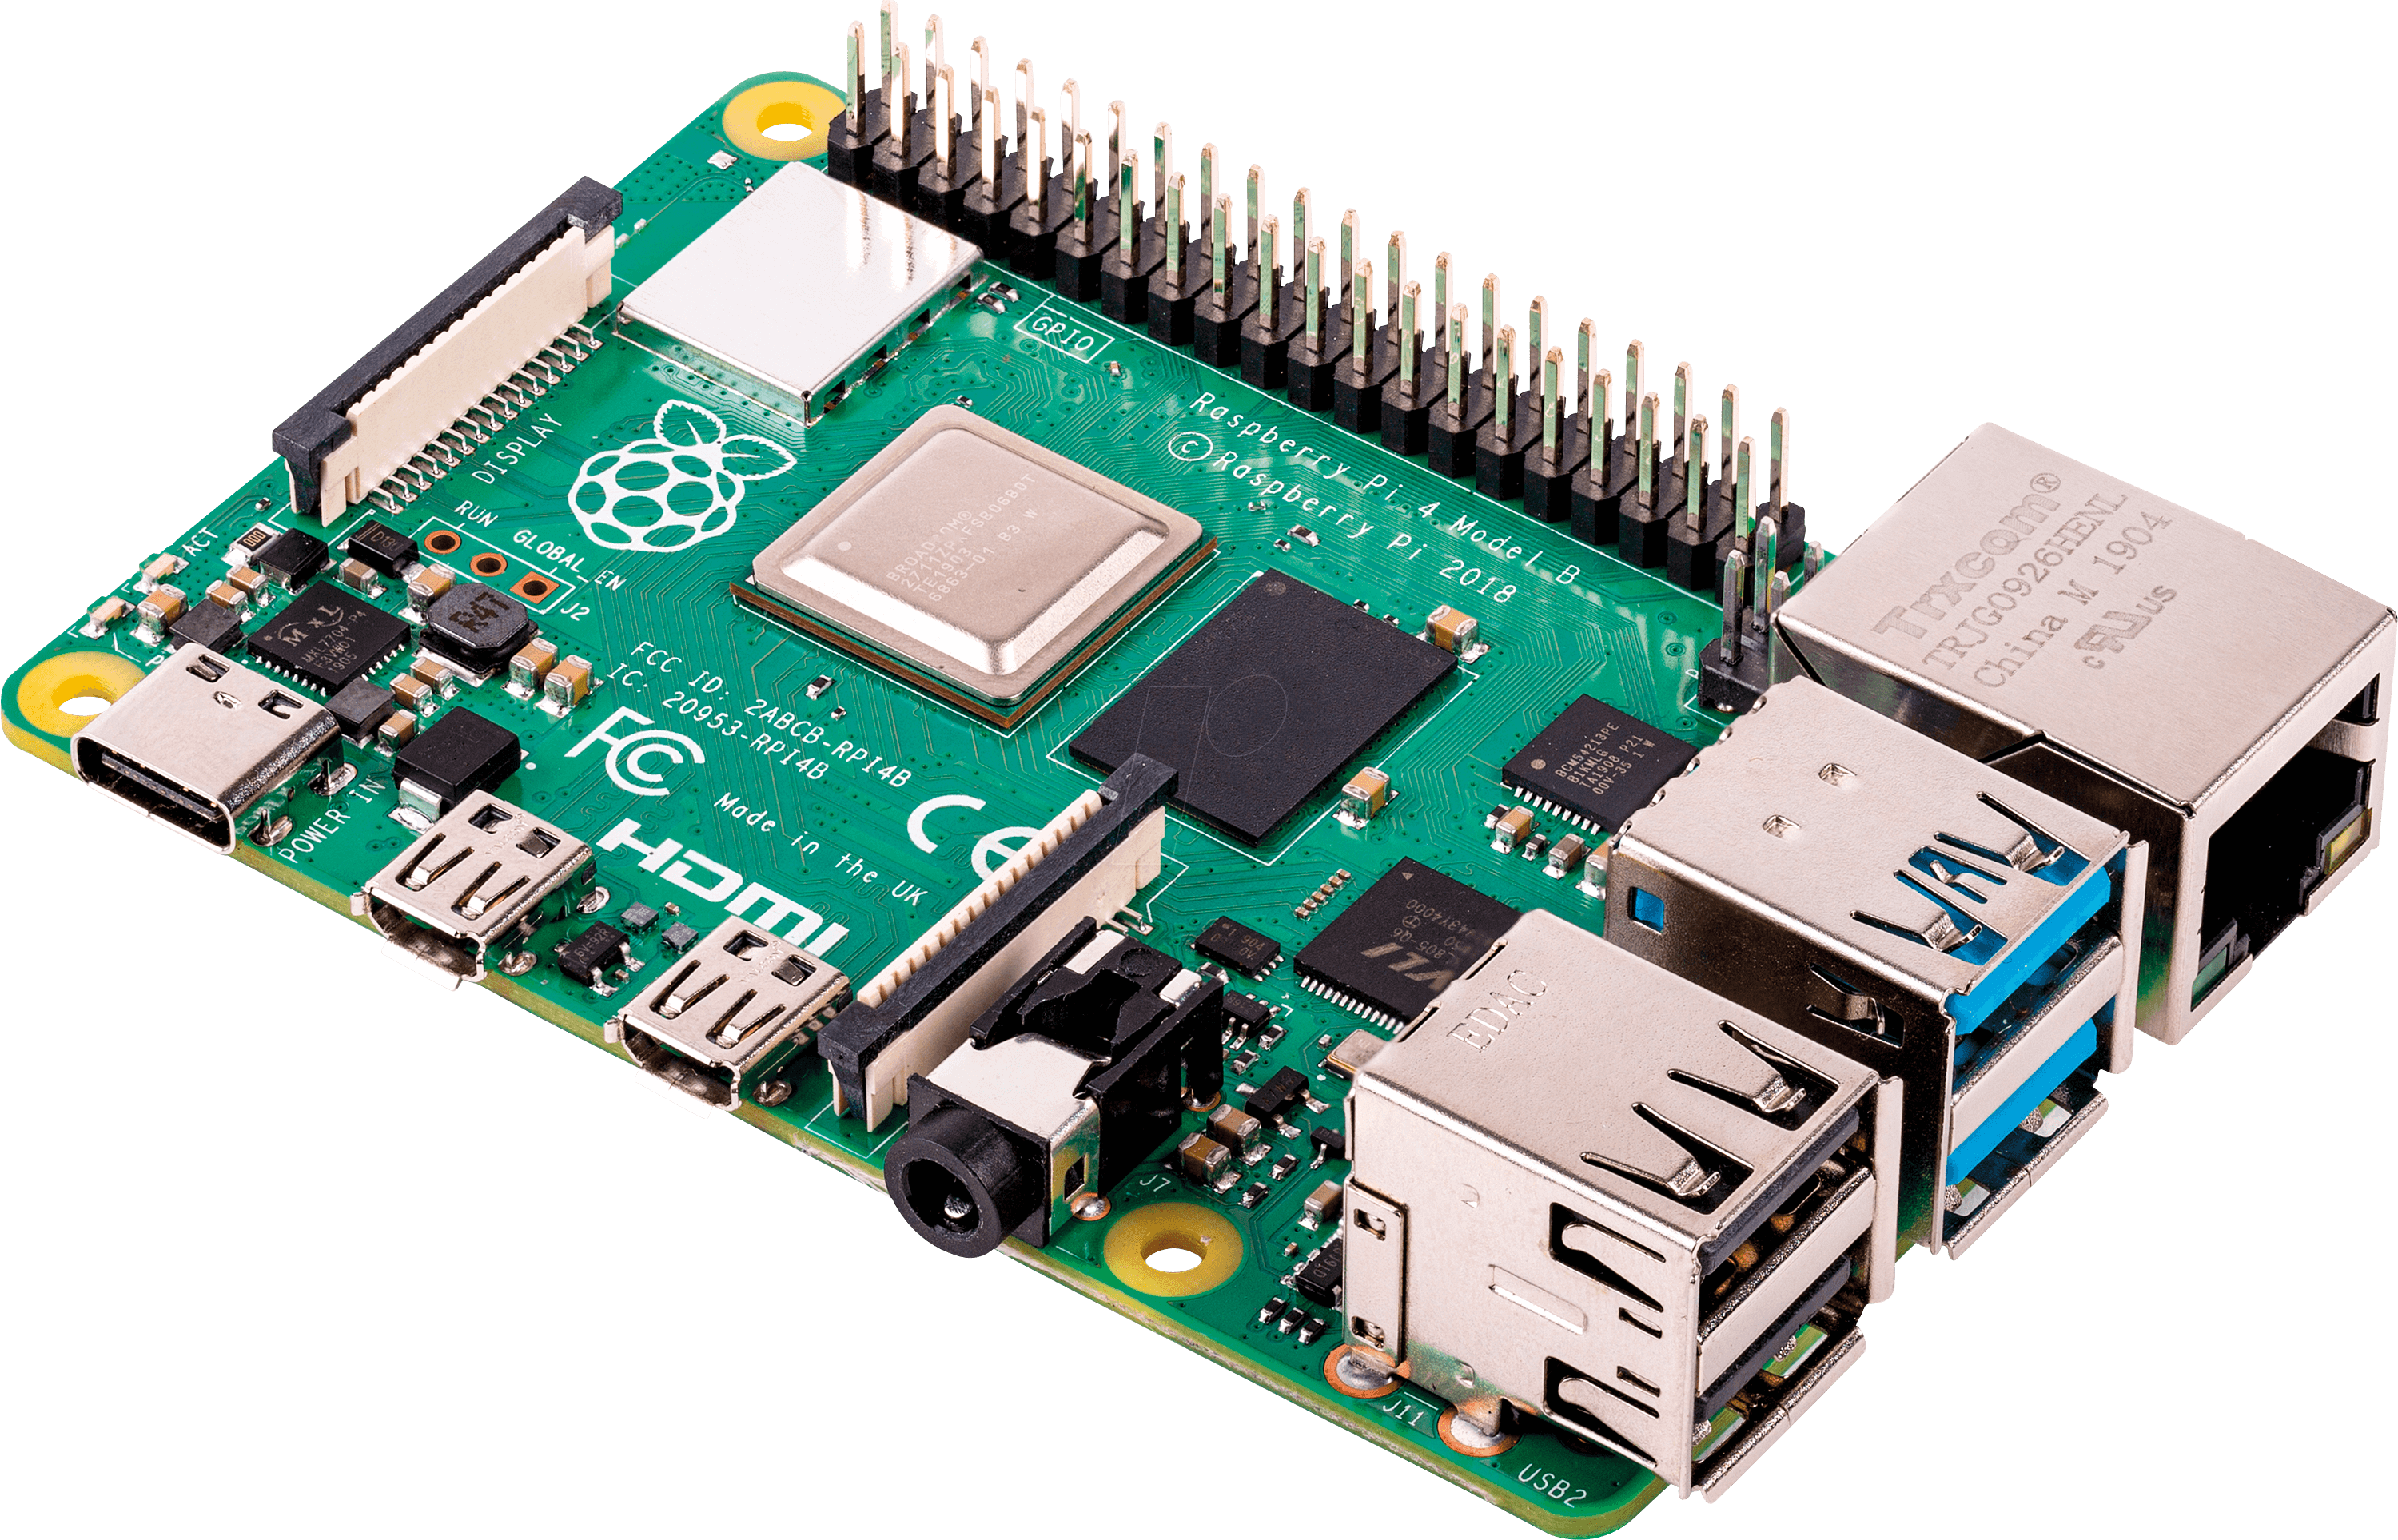
\includegraphics[scale=0.08]{figures/hcis/raspberryPi.png}
		\caption{Raspberry Pi - Steuereinheit des HCIS}
	\end{center}
\end{figure}

\subsection{Grundaufbau des Systems}

In der Abbildung \ref{fig:aufbauHCIS} wird der Grundaufbau des Systems und die Datenverbindungen der folgenden  Komponenten veranschaulicht.

\begin{itemize}
	
	\item Raspberry Pi - Die Steuereinheit des Systems.
	\\ Kommuniziert über CAN-Bus mit den anderen Steuerkomponenten des Motorrades.
	
	\item User Input - Die vorhandenen Schalter am Lenker des Motorrads werden direkt mit den Eingängen des Raspberry Pis verbunden. 
	
	\item Peripherie - Die Grundkomponenten des Motorrades wie Scheinwerfer oder Hupe. Diese werden über Relais, welche an die Ausgänge des Raspberry Pis angeschlossen sind, gesteuert.
	
	\item Dashboard - Der Bildschirm zur Anzeige der verarbeiteten Informationen. Dieser wird über HDMI und USB mit dem Raspberry Pi verbunden.
	
\end{itemize}

\begin{figure}[H]
	\begin{center}
		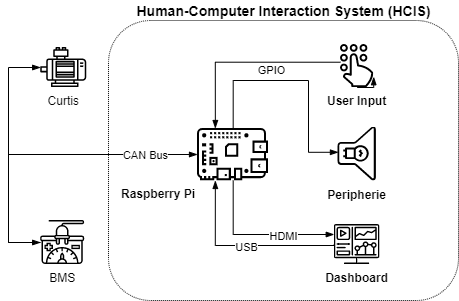
\includegraphics[scale=0.5]{figures/hcis/HCIS_Grundfunktion.png}
		\caption{Grundaufbau des Human-Computer Interaction Systems}
		\label{fig:aufbauHCIS}
	\end{center}
\end{figure}

Nicht in der Abbildung dargestellt ist die Versorgung der einzelnen Komponenten, welche in dem folgenden Abschnitt noch genauer erläutert wird.

\newpage


%% Versorgung %%%%%%%%%%%%%%%%%%%%%%%%%%%%%%%%%%%%%%%%%%%%%%% 

\section{Spannungsversorgung}

\subsection{Aufbau des Versorgungssystems} \label{sec:aufbauversorgung}

Das Versorgungssystem des Motorrades besteht aus zwei Spannungsebenen: Einer 12V Ebene zur Versorgung der Peripherie des Motorrades und einer 5V Ebene, welche nur den Raspberry Pi und seine Komponenten beinhaltet. Diese Ebenen werden durch DC-DC Wandler erzeugt, welche direkt an den Akku des Motorrades angeschlossen werden. \\

Wichtig hierbei ist, dass alle ausgewählten Spannungswandler über einen Kurzschluss- und Überstrom-Schutz verfügen. Dies macht es uns möglich diese Versorgungssysteme, solange die Drähte auch nach dem maximalen Strom der Spannungswandler dimensioniert wurden, ohne jegliche Leitungs- und Überstrom-Schutzorgane aufzubauen. Die Spannungswandler schalten bei jeglichen Fehlern ab und verbrennen die überschüssige Leistung über einen eingebauten Widerstand. Sobald der Fehler behoben wurde, schalten sich die Spannungswandler automatisch wieder ein.

\subsubsection{12V Versorgungsysstem}

Um den Spannungswandler dimensionieren zu können mussten vorher alle Bauteile, welche über die 12V versorgt werden sollten, zusammengefasst werden, um die mindestens benötigte Leistung des Spannungswandlers zu errechnen. 

\begin{table}[H]
	\begin{center}
		\begin{tabular}{|l|c|c|}
			\hline
			\textbf{Bauteilbezeichnung}     & \textbf{Spannung} & \textbf{Leistung} \\ \hline
			Tagfahrlicht           & 12V      & 10W      \\ \hline
			Abblendlicht           & 12V      & 10W      \\ \hline
			Aufblendlicht          & 12V      & 20W      \\ \hline
			Hupe                   & 12V      & 10W      \\ \hline
			Rücklicht              & 12V      & 21W      \\ \hline
			Kennzeichenbeleuchtung & 12V      & 5W       \\ \hline
			Blinker links          & 12V      & 2 x 10W  \\ \hline
			Blinker rechts         & 12V      & 2 x 10W  \\ \hline
			Bildschirm             & 12V      & 12W      \\ \hline
			\textbf{Gesamt}                 & \textbf{12V}      & \textbf{128W}     \\ \hline
		\end{tabular}
			\caption{Berechnung der Leistung des 12V-Systems}
			\label{tab:leistung12V}
	\end{center}
\end{table}

Der Spannungswandler wurde nun nach der größt möglichen Leistung, welche auftritt wenn alle Bauteile gleichzeitig auf Höchstleistung betrieben werden, ausgelegt. Diese maximale Leistung beträgt, wie in der Tabelle \ref{tab:leistung12V} zu sehen, 128 Watt. Um noch Ausbaumöglichkeiten zu gewährleisten und uns nicht dem Leistungslimit des Wandlers zu nähern, haben wir uns für einen 48V-12V, 300 Watt DC-DC Wandler von Mean Well \footnote{Datenblatt: siehe Anhang \ref{app:mw12}} entschieden. 

\subsubsection{5V Versorgungssystem}

Die Leistung des Raspberry Pis ist mit einem Maximum von 6.2 Watt sehr klein und daher ist die Wahl des Spannungswandlers in diesem Fall nicht wirklich davon abhängig. Auch die Komponenten, welche angeschlossen werden, haben grundsätzlich keine erwähnenswerte Wirkleistung und müssen daher nicht genau ein berechnet werden. Nun entschied nur mehr das Preis-Leistungs-Verhältnis sowie die Ausfallsicherheit des Spannungswandlers die Wahl. Daher haben wir uns für einen 48V-5V, 30 Watt DC-DC Wandler von Meanwell \footnote{Datenblatt: siehe Anhang \ref{app:mw5}} entschieden.

\subsubsection{Abschalten der Spannungswandler}

Das Abschalten der Spannungswandler ist nicht notwendig, da diese - wie schon in Abschnitt \ref{sec:aufbauversorgung} erklärt - bei einem anliegenden Fehler automatisch abschalten.
Ebenso wird beim Abschalten des Motorrades über die BMS jegliches andere Bauteil von der Spannungsversorgung getrennt. Was die Spannungswandler vom Entladen des Akkus abhält.  

\newpage

%% Steuerung der Peripherie %%%%%%%%%%%%%%%%%%%%%%%%%%%%%%%%%

\section{Steuerung der Peripherie}

Die Grundfunktionen wie Beleuchtung, Hupe und Blinker werden hier als Peripherie bezeichnet. Diese sollten so einfach wie möglich und vom Lenker aus zu bedienen sein. Ebenso müssen sie verlässlich gesteuert werden können. Daher haben wir uns entschieden diese Funktionen ebenso über den Raspberry Pi zu steuern, da dieser bei einem Fehler der Motorsteuerung über den eingebauten Puffer gespeist werden kann und daher diese wichtigen Funktionen bis zu einem sicheren Stillstand weiter betrieben und gesteuert werden können.\\


Dennoch ist in der Plan in Zukunft die Motorsteuerung, welche ebenso in der Lage wäre die Ausgänge abhängig von den Eingängen zu schalten, diese Aufgabe übernehmen zu lassen, solange die Ausfallsicherheit ebenso gegeben wäre. Der Vorteil dieser Methode ist die Schaffung einer Zentralen Steuereinheit, welche alle Steueraufgaben in einem Bauteil vereinen kann.

\subsection{Hardware}

\subsubsection{Input}

Man kann einen GPIO Pin entweder als Eingang oder als Ausgang betreiben. Als Eingang kann er die Zustände High und Low einnehmen. Zum Beispiel von einem Schalter oder Taster. In der Regel beschaltet man die GPIOs des Raspberry Pis mit Widerständen, um Eingänge auf einen definierten Pegel zu setzten oder um den Strom zu begrenzen. Standardmäßig werden 10k Widerstände benutzt. Ob Pullup oder Pulldown ist grundsätzlich gleichgültig. Wir benutzen für das Einlesen der Eingänge 10k Pulldown Widerstände, um nicht immer eine Spannung an den Eingängen des Raspberry Pis anliegen zu haben.

\begin{figure}[H]
	\begin{center}
		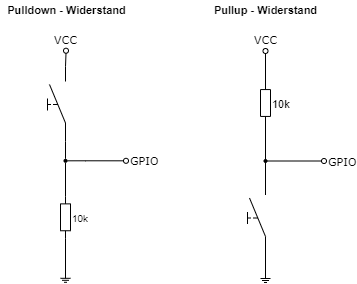
\includegraphics[scale=0.8]{figures/hcis/input.png}
			\caption{Anschlussplan Eingänge}
			\label{fig:input}
	\end{center}
\end{figure}

\textbf{Pullup Widerstand}\\

Bei dem Nutzen eines Pullup Widerstands wird der GPIO Pin mit einem Widerstand auf die Spannnung von VCC gezogen. Der Grundzustand des Eingangs ist dann High. Mit einem Schalter oder Taster wird der Eingang dann gegen Ground gezogen. Das heißt er hat solange der Schalter geschlossen ist, liegt das Massepotential am Eingang an.\\\medskip

\textbf{Pulldown Widerstand}\\

Bei dem Nutzen eines Pulldown Widerstands wird der GPIO Pin mit einem Widerstand auf die Spannnung von Ground gezogen. Der Grundzustand des Eingangs ist dann Low. Mit einem Schalter oder Taster wird der Eingang dann gegen VCC gezogen. Das heißt er hat solange der Schalter geschlossen ist, liegt das Versorgunspotential am Eingang an.

\subsubsection{Output}

Hierbei werden die GPIOs als Ausgang verwendet. Sie sind verbunden mit den Eingängen eines 4 Channel Relais Moduls, welches über die 5V direkt von dem Raspberry Pi gespeist wird. Hiermit ist es nun Möglich die 12V der Perpherie zu schalten und 

\begin{figure}[H]
	\begin{center}
		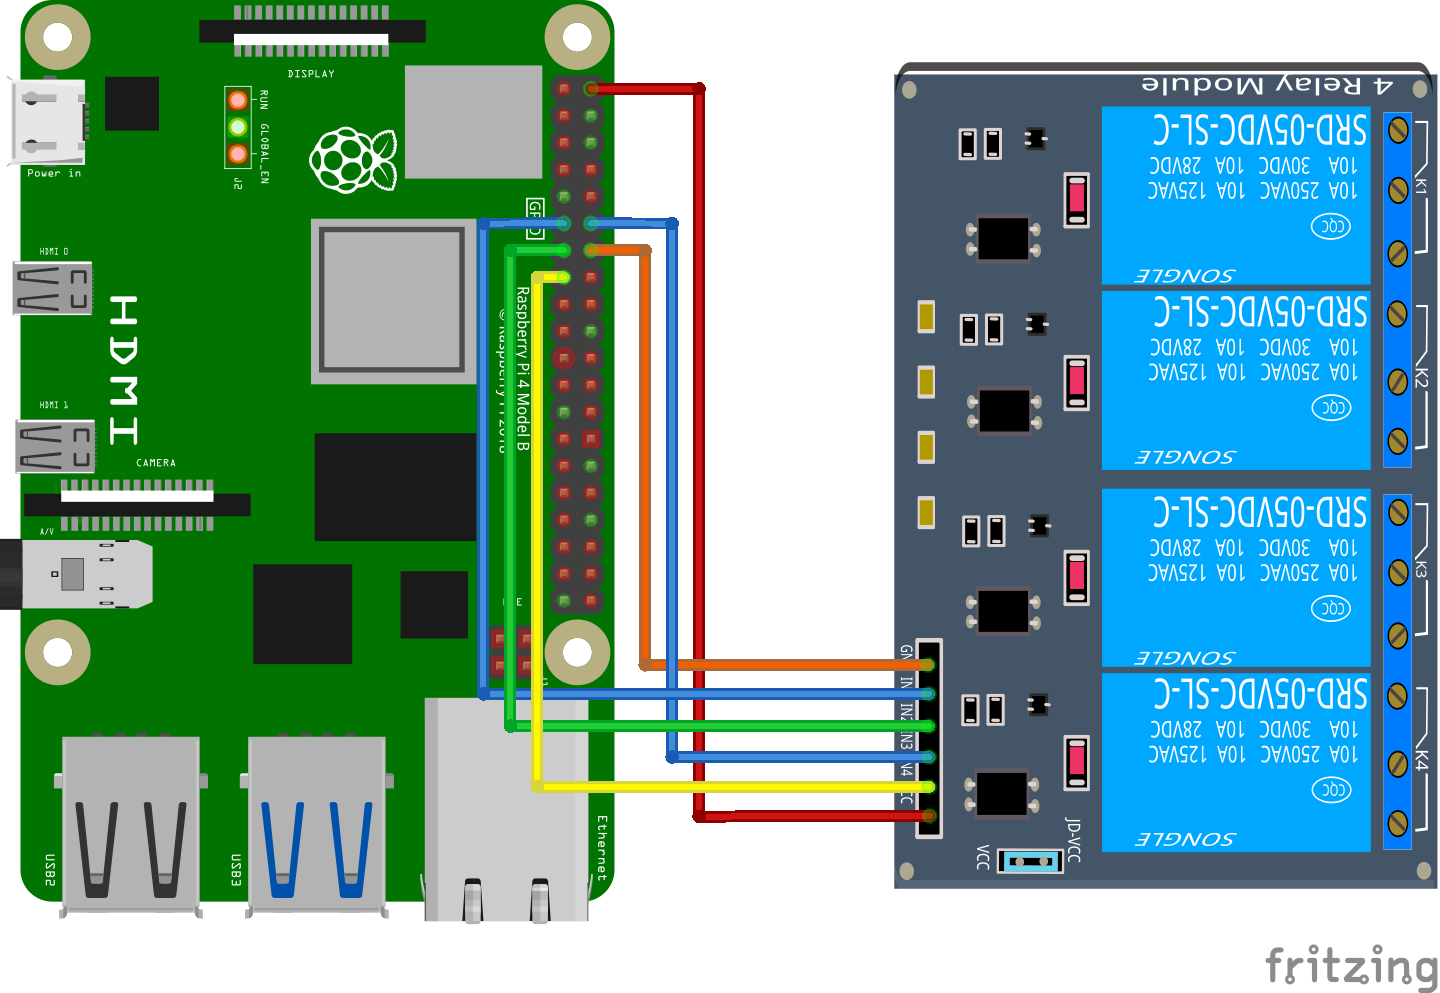
\includegraphics[scale=0.7]{figures/hcis/4ch_relai.png}
			\caption{Anschlussplan Relais}
			\label{fig:output}
	\end{center}
\end{figure}

\subsection{Software}

Wichtig bei der Programmierung war in diesem Fall die dauerhafte Verfügbarkeit der Grundfunktionen  sowie die einfache Integrierbarkeit von alten und neuen Bauteilen. Dies wurde erreicht durch die Anwendung verschiedener Bibliotheken.\\
Die Wichtigsten in dieser Anwendung waren: \\

\subsubsection{gpiozero}

Eine Bibliothek, welche das einfache und schnelle Integrieren neuer Ein- oder Ausgänge ermöglicht. Dadurch können schnell und einfach Änderungen an dem Steuerverhalten der Peripherie gemacht werden. Hierzu kann die Klasse Button und DigitalOutputDevice verwendet werden. Dieser können Parameter wie die gewünschte Debounce Zeit und verwendete Pull-Widerstände übergeben werden. Es werden nur drei Zeilen Code benötigt um einen Aus- oder Eingang zu definieren und anzusteuern \footnote{siehe: Anhang}

\subsubsection{threading}

Eine Bibliothek, welche es ermöglicht, einen eigenen Thread \footnote{gleichzeitig laufende Aufgabe} für das Programm zu öffnen, wodurch die Anwendung ohne Einflüsse oder Unterbrechungen anderer Programme weiter arbeiten kann. Der folgende Programmcode zeigt einen Ausschnitt der Klasse zum Steuern der GPIOs. 

\begin{lstlisting}[language=Python, caption={Code zum Starten eines Threads},captionpos=b]
	
	def start(self):
		self.thread=Thread(target=self.runner)
		self.thread.daemon=True
		self.thread.start()

\end{lstlisting}

In diesem Beispiel wird ein Demon Thread erzeugt und gestartet. Das beutetet dieser Thread wird beim schließen des Programms automatisch mit geschlossen und muss dadurch nicht mehr überwacht werden. Das Target ist die Funktion, welche unabhängig ausgeführt werden soll.

\newpage

%% Benutzeroberfläche %%%%%%%%%%%%%%%%%%%%%%%%%%%%%%%%%%%%%%%

\section{Benutzeroberfläche}
Die Benutzeroberfläche stellt die Verbindung zwischen dem Nutzer und dem Motorrad dar. Sie sollte während der Fahrt die Instrumententafel des Motorrades ersetzen und dem Nutzer die wichtigsten Fahrinformationen anzeigen. Sobald das Motorrad zum Stillstand gekommen ist, wird es möglich Einstellungen zu ändern und die aufgezeichneten Fahrdaten anzeigen zu lassen. Ebenso können der Akkuladestatus und Informationen über Fehler im System entnommen werden.

\subsection{Hardware}

Zur Anzeige und Bedienung wird ein 11.6 Zoll kapazitives Touch LCD Display verwendet. Es besitzt eine Full HD Auflösung (1920x1080), was für eine professionelle Darstellung essentiell ist. Ebenso hat es ein schützendes ABS Gehäuse, welches trotz fehlender IP Zertifizierung das Abdichten ermöglicht. Die Versorgungsspannung beträgt 12V, was ident zu den anderen Komponenten am Motorrad ist und daher die Versorgung sehr vereinfacht, es kann also über den gleichen Spannungswandler versorgt werden.

\begin{figure}[H]
	\begin{center}
		\includegraphics[scale=0.45]{figures/hcis/display_maße.png}
		\caption{Paneel Maße}
		\label{fig:panel}
	\end{center}
\end{figure}

Die Auflösung und die Größe des Paneels wirkt sich stark auf das Design der Benutzeroberfläche aus. Es muss die Größe der Icons und der anderen Designelemente so angepasst werden, dass sie einerseits gut ersichtlich und andererseits einfach über Berührung zu bedienen sind.\\

\newpage

\subsubsection{Befestigung}
Besser: In das Gehäuse des Paneels sind M4 Verschraubungen in einem Raster von 75mm x 75mm integriert und kann daher einfach an Wänden oder Platten verschraubt werden. Um den Bildschirm nun in einer ähnlichen Position wie die Instrumententafel zu befestigen wurde eine 100mm x 210mm x 1.5mm Aluminium Platte - wie in der Abbildung zu sehen - gebogen und mit Löchern versehen. Um diese Halterung nun an dem Motorrad zu befestigten werden die Verschraubungen der alten Instrumententafel verwendet.

\begin{figure}[H]
	\begin{center}
		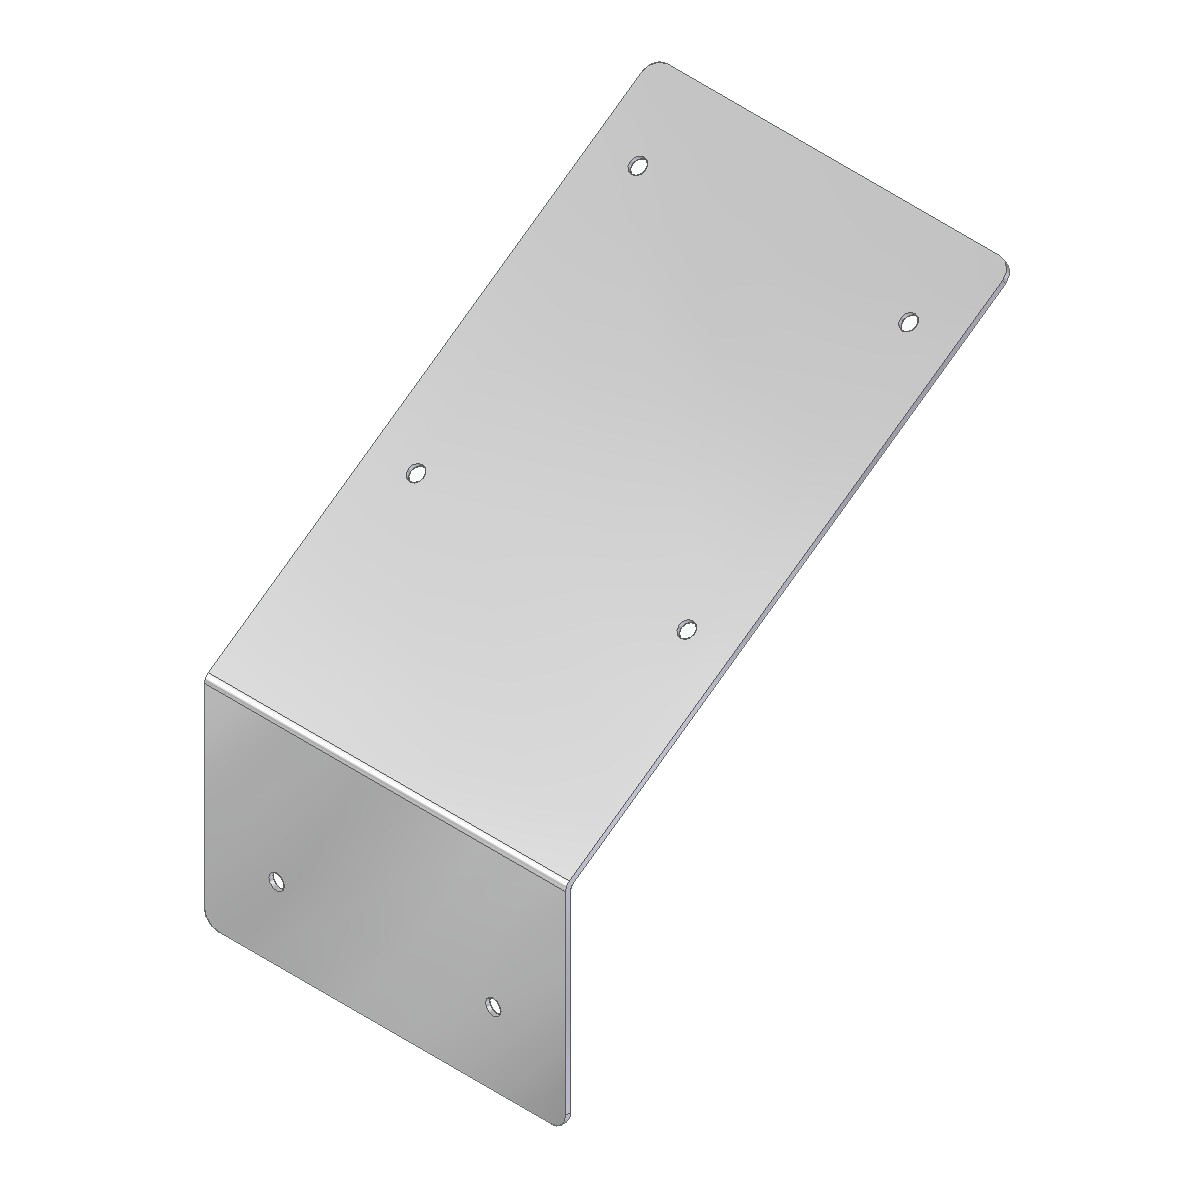
\includegraphics[scale=0.18]{figures/hcis/befestigung_display.png}
		\caption{Befestigung des Displays}
		\label{fig:befestigung}
	\end{center}
\end{figure}

\subsection{Software}
Bevor die Software für die Benutzeroberfläche verfasst wurde, mussten das Design, die Funktionen sowie die angezeigten Informationen geplant werden, um einen reibungslosen Arbeitsablauf beim Entwickeln des Frontends zu gewährleisten. Design Elemente wurden zuvor in Adobe Illustrator vorgefertigt. In den folgenden Seiten wird das Ergebnis dieses Prozesses erläutert.
\subsubsection{Aufbau}
Die nachfolgende Abbildung zeigt den grundsätzlichen Programmaufbau der Benutzeroberfläche. Die einzelnen Fenster werden als Tabelle mit ihren angezeigten Informationen dargestellt. Dies is wichtig da jede dieser Informationen vom Backend an das Frontend gesendet werden müssen.\\
Ebenso sind in den letzten Zeilen der Tabellen die QML-Elemente  zur Navigation zwischen den einzelnen Fenstern niedergeschrieben. Diese müssen auch schon in der frühen Phase der Entwicklung der Benutzeroberfläche definiert werden.

\begin{figure}[H]
	\begin{center}
		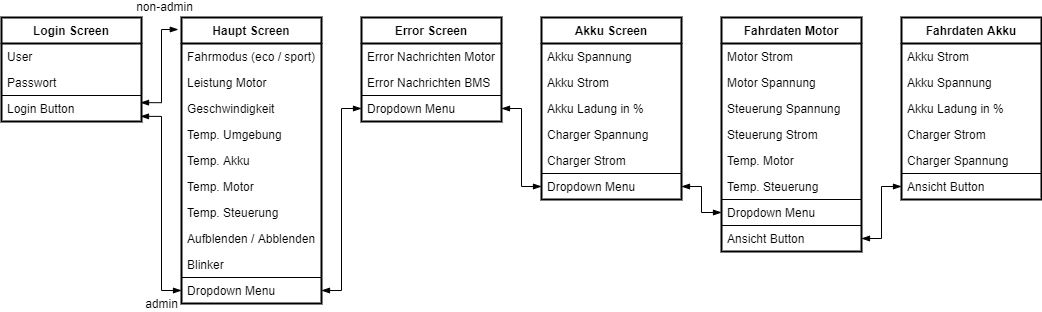
\includegraphics[scale=0.4]{figures/hcis/gui_aufbau.png}
		\caption{Aufbau der Graphischen Benutzeroberfläche}
		\label{fig:aufbauGUI}
	\end{center}
\end{figure}

\newpage

\subsubsection{Nutzer / Berechtigungen}

\subsection{Komponenten}

Komponenten sind wiederverwendbare, gekapselte QML-Elemente mit genau definierten Schnittstellen. Komponenten werden häufig durch Komponenten-Dateien definiert, das heißt durch QML-Dateien. Wichtig ist dabei die Definition von Schnittstellen sowie Properties und Signals .

\textbf{Properties}\\
\vspace{2mm}

Einer Property eines Objektes kann ein statischer Wert zugewiesen werden, der konstant bleibt, bis ihm explizit ein neuer Wert zugewiesen wird. Um QML und seine integrierte Unterstützung für dynamisches Objektverhalten optimal zu nutzen, verwenden die meisten QML-Objekte jedoch Propertysbindings.\\
Dies sind eine Kernfunktion von QML, mit der Beziehungen zwischen verschiedenen Objekteigenschaften festgelegt werden können. Wenn sich die Abhängigkeiten einer Property im Wert ändern, wird die Eigenschaft automatisch gemäß der angegebenen Beziehung aktualisiert.\\
Hinter den Kulissen überwacht die QML-Engine die Abhängigkeiten der Eigenschaft. Wenn eine Änderung erkannt wird, wertet die QML-Engine den Bindungsausdruck erneut aus und wendet das neue Ergebnis auf die Eigenschaft an.

\textbf{Java-Script-Funktionen}\\
\vspace{2mm}

Programmlogik kann auch in Java-Script-Funktionen definiert werden. Diese können in QML-Dokumenten definiert und von Signalhandlern, Eigenschaftsbindungen oder Funktionen in anderen QML-Objekten aufgerufen werden. Solche Methoden werden häufig als Inline-Java-Script-Funktionen bezeichnet, da ihre Implementierung im QML-Dokument statt in einer externen Java-Script-Datei enthalten ist.

\subsubsection{Navigationsmenü}

Das Navigations-Menü ist ein Dropdown-Menü, welches zur Navigation zwischen den verschiedenen Fenstern benützt wird. Sobald man sich eingeloggt hat wird das Menü angezeigt und die einzelnen Untermenüs können aufgerufen werden. Das Menü wird abhängig von den Berechtigungen des Benutzers angepasst.

\begin{figure}[H]
	\begin{center}
		
\includegraphics[scale=0.2]{figures/hcis/component_menu.png}
		\caption{GUI Komponente - Navigation Menü}
		\label{fig:kompNavigation}
	\end{center}
\end{figure}

\textbf{Buttons} \\
\vspace{2mm}
Die Navigation wird über das QML-Element \textit{Mousearea}, welche direkt über den Icons der einzelnen Navigationselemente platziert wurde, gesteuert. Nun kann mit dem Befehl \textit{onClicked} eine Funktion aufgerufen werden, welche das gewünschte Fenster sichtbar macht, sowie das Navigationsmenü wieder nach oben fahren lässt.\\
In dieser Funktion wird ebenso die Berechtigung des Nutzers über eine Globale Variable, welche beim Anmelden durch ein Signal gesetzt wird, abgefragt. Falls die Berechtigung die ausgewählte Funktion nicht zulässt wird ein Informationstext ausgegeben und das Menü wiederum geschlossen.\

\textbf{Abmelden} \\
\vspace{2mm}

Wird der Abmeldebutton gedrückt, werden die Anmeldeinformationen zurückgesetzt und dem Nutzer wird wieder das Anmeldefenster angezeigt, wo er sich nun mit anderen Anmelde-Informationen einloggen kann.

\newpage

\subsubsection{Balken Anzeige}

Die Komponente Balken Anzeige wird in der Benutzeroberfläche zur Visualisierung verschiedener Daten verwendet. Mit ihr können diese übersichtlicher Dargestellt werden. Diese Komponente wird in mehreren QML-Dateien verwendet, daher sind Properties zur Anpassung notwendig. Die wichtigsten davon sind:

\begin{itemize}
	\item Wert - Der Aktuelle Wert, welcher am Balken angezeigt werden sollte.
	\item Anfangswinkel - Der Winkel an dem der Balken entspringt.
	\item maximaler Wert - Der maximal zu erreichende Wert. Dieser Bestimmt die Länge des Hintergrundbalkens
	\item Hintergrundfarbe - Farbe des Hintergrundbalkens (in der Abbildung grau)
	\item Balkenfarbe -Farbe des Anzeigebalkens (in der Abbildung blau)
\end{itemize}

\begin{figure}[H]
	\begin{center}
		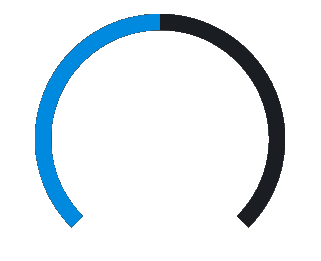
\includegraphics[scale=0.5]{figures/hcis/component_bar.png}
		\caption{GUI Komponente - Balken Anzeige}
		\label{fig:kompBalken}
	\end{center}
\end{figure}

Über ein \textit{Signal} kann nun über das Backend der Wert des Balkens verändert werden und in Echtzeit angezeigt werden.

\subsubsection{Modus Anzeige}
Diese Komponente befindet sich auf der Instrumenten Tafel. Der Modus kann über einen Button am Lenker, welcher mit der Curtis Steuerung verbunden ist, geändert werden. Sie dient zum Anzeigen der derzeitig gewählten Fahrmodi und wird über ein \textit{Signal} aus dem Backend gesteuert, welches mit der Listener Klasse verbunden ist.

\begin{figure}[H]
	\begin{center}
		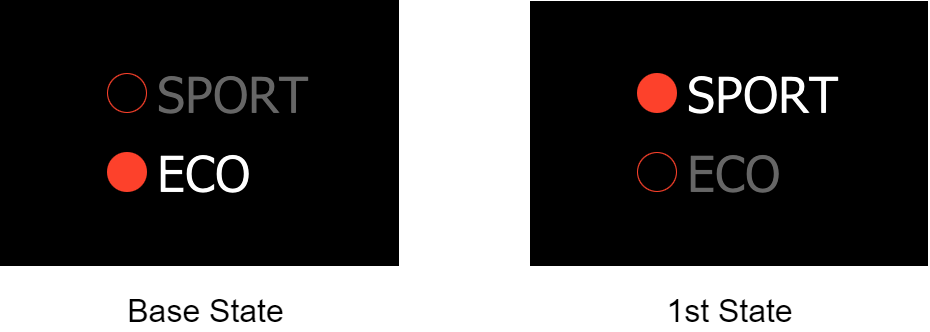
\includegraphics[scale=0.4]{figures/hcis/component_mode.png}
		\caption{GUI Komponente - Modus Anzeige}
				\label{fig:kompModus}
	\end{center}
\end{figure}

Die Modus Anzeige ist eine einfache Komponente. Sie ist ein Item QML-Typ, dadurch wird das Nutzen von \textit{States} möglich. Durch diese können verschiedene Eigenschaften gespeichert und über einen kurzen Befehl wiederhergestellt werden.\\
In diesem Fall wird der Punkt ausgefüllt und die Farbe des Textes geändert.

\newpage

\subsubsection{Graph} \label{sec:graph}

Die Graph Komponente befindet sich auf dem Diagnose Fenster und dient zum Anzeigen der in der Datenbank gespeicherten Fahrdaten. Sie verfügt über einen Ladebalken, welcher nach dem Auswählen der anzuzeigenden Daten den Fortschritt des Auslesens der Datenbank anzeigt. Dieses Auslesen läuft über eine Funktion der Fetcher Klasse.

\begin{figure}[H]
	\begin{center}
		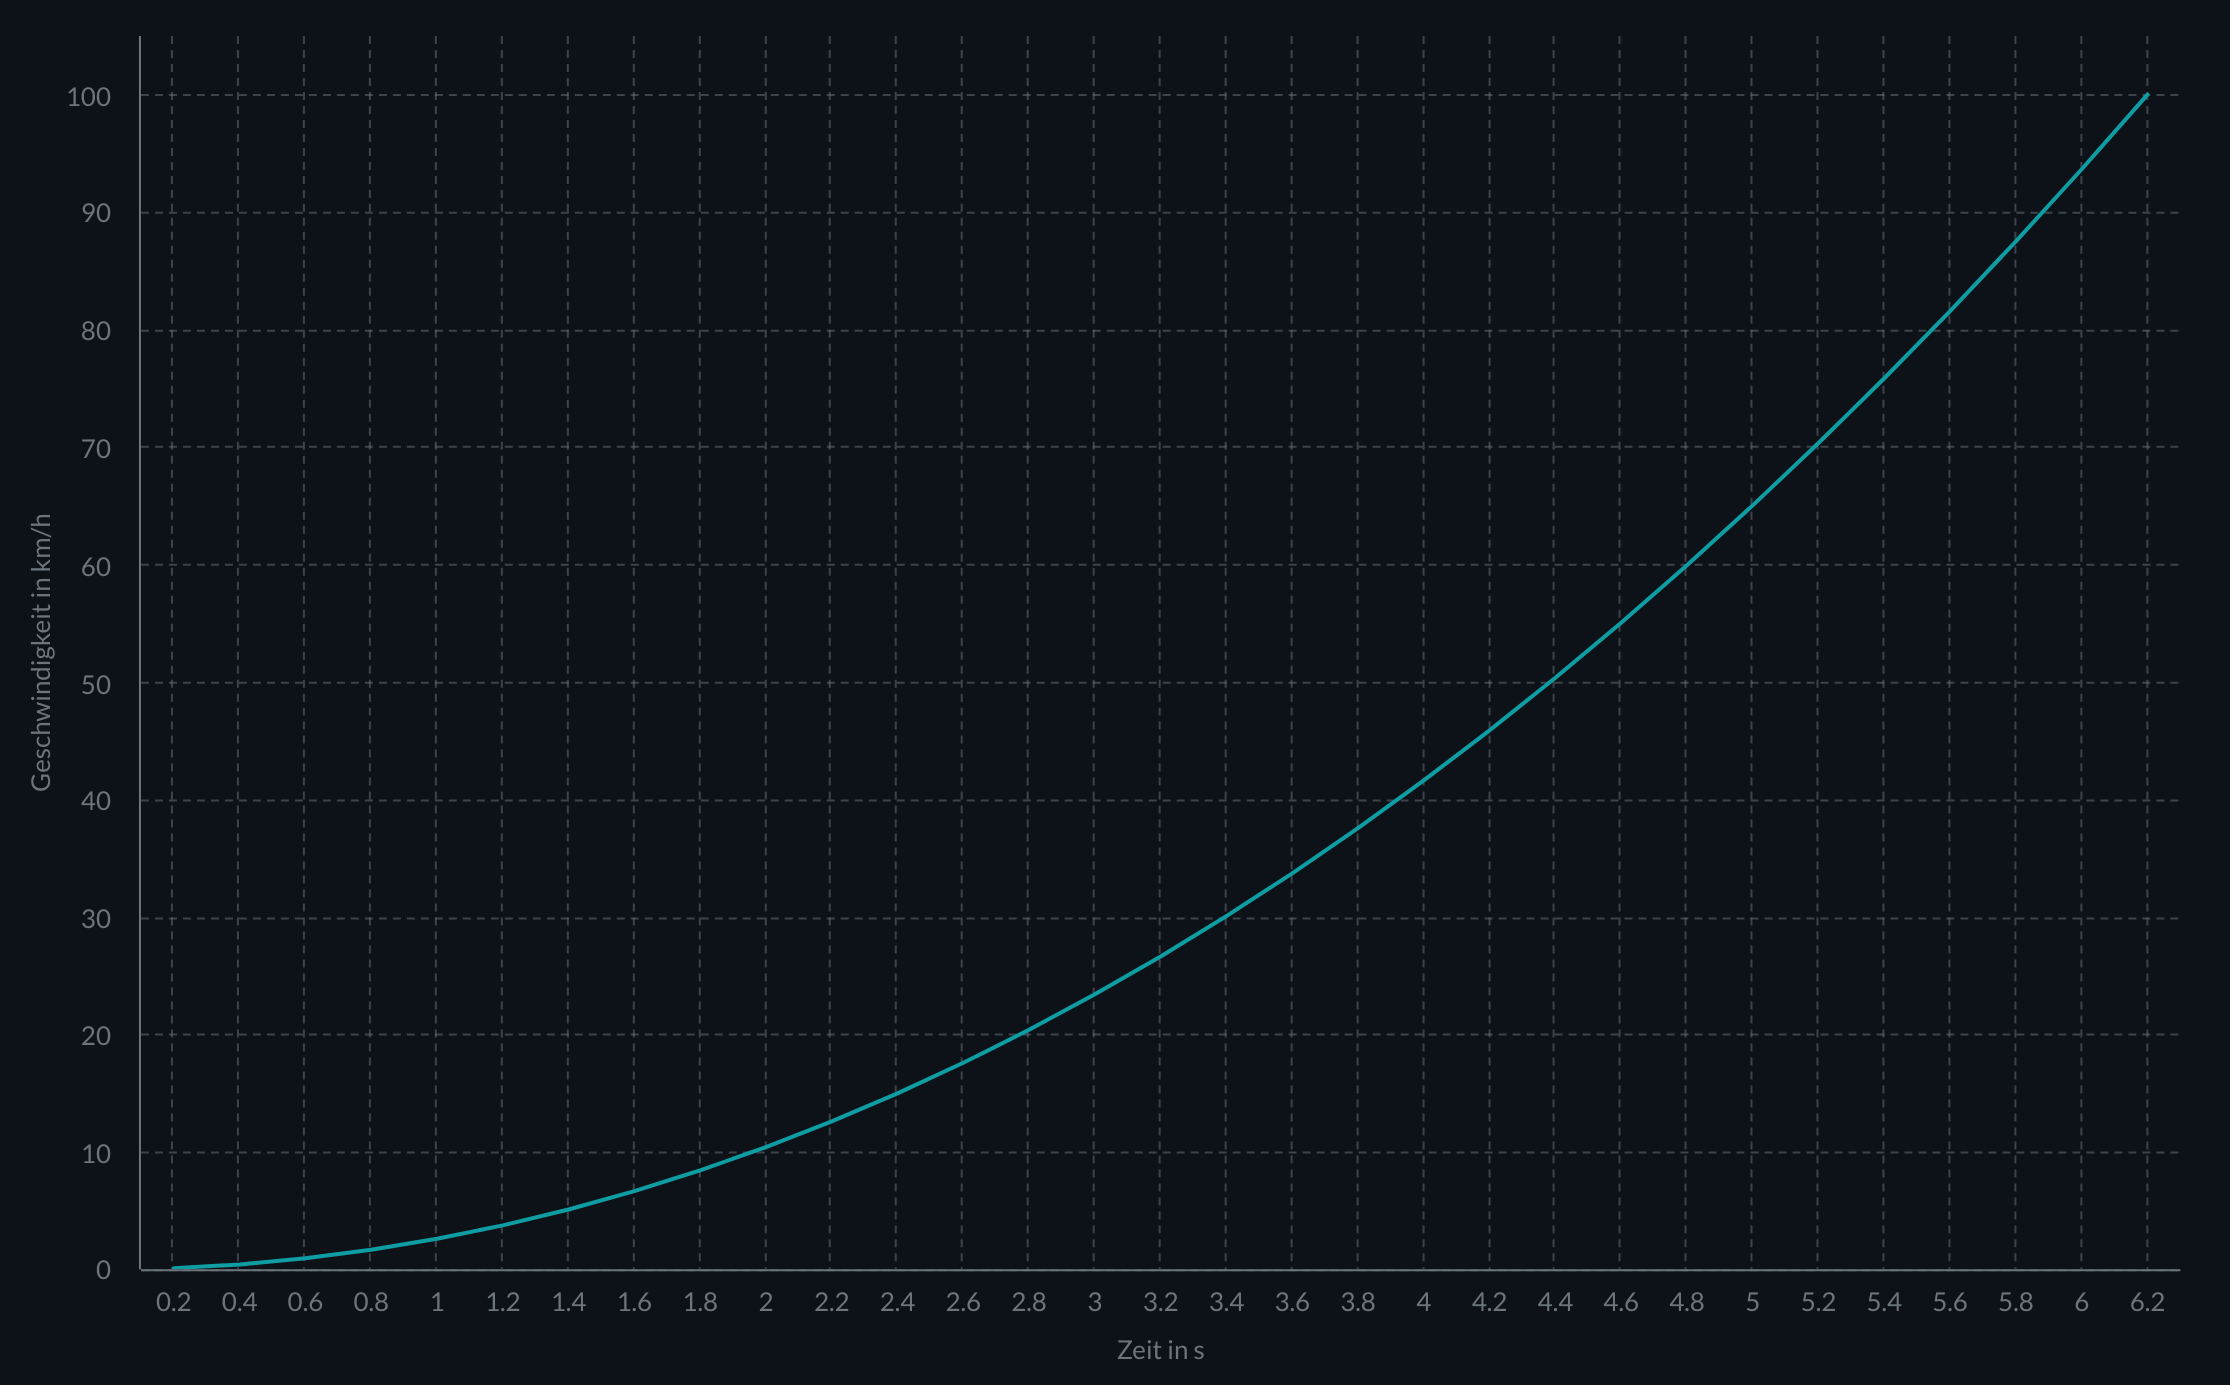
\includegraphics[scale=0.3]{figures/hcis/component_graph.png}
		\caption{GUI Komponente - Graph}
				\label{fig:kompGraph}
	\end{center}
\end{figure}

Realisiert wurde diese Komponente über öffentliche Bibliothek \textit{Charts.js} (Referenz), welche durch die Java Script Unterstützung von \textit{QT}, mit der Installation eines Adapters mit dem QML Programm kompatibel ist. Dadurch wird nun das Zeichnen von verschiedensten Graphen ermöglicht.

\subsubsection{Weitere Komponenten}

Wie schon bei der Fahr Modi Komponente, wurden weitere Objekte, welche zwischen zwei Zuständen hin und her gestalten werden müssen oder eine bestimmte Handlung ausführen sollten, über eine eigene QML Komponente verwirklicht. Diese Ermöglicht nun wiederum das wiederholte verwenden dieser Komponente, sowie das Ansteuern über \textit{States} und \textit{Signale}.\\
Diese Komponenten sind:

\textbf{Umschaltkomponenten}\\
Dies sind Komponenten, welche über ein \textit{Signal} angesteuert werden und dann mithilfe von \textit{States} ihr Aussehen verändern.

\begin{itemize}
	
	\item Blinker Rechts
	\item Blinker Links
	\item Tagfahrlicht
	\item Fernlicht
	
\end{itemize}

\textbf{Touch Komponenten}\\
Dies sind Komponenten, welche eine \textit{Mousearea} mit einer Graphik verbindet. Wird diese Komponente nun mit einem Mausklick ausgewählt, kann eine Funktion ausgeführt oder ein \textit{Signal} ausgesendet werden.

\begin{itemize}
	
	\item Abmeldebutton
	\item Navigationsmenübuttons
	\item Menü-Öffnen-Button
	
\end{itemize}

\newpage

\subsection{Programm Fenster}

\subsubsection{Login}

Das Login Fenster dient zur Autorisierung des Benutzers. Über die User \textit{Kombobox} kann der gewünschte Nutzer mit der dazugehörigen Berechtigung ausgewählt werden (siehe Abschnitt ). Das Fenster dient ebenso zur Darstellung der Logos unserer Sponsoren\\

\begin{figure}[H]
	\begin{center}
		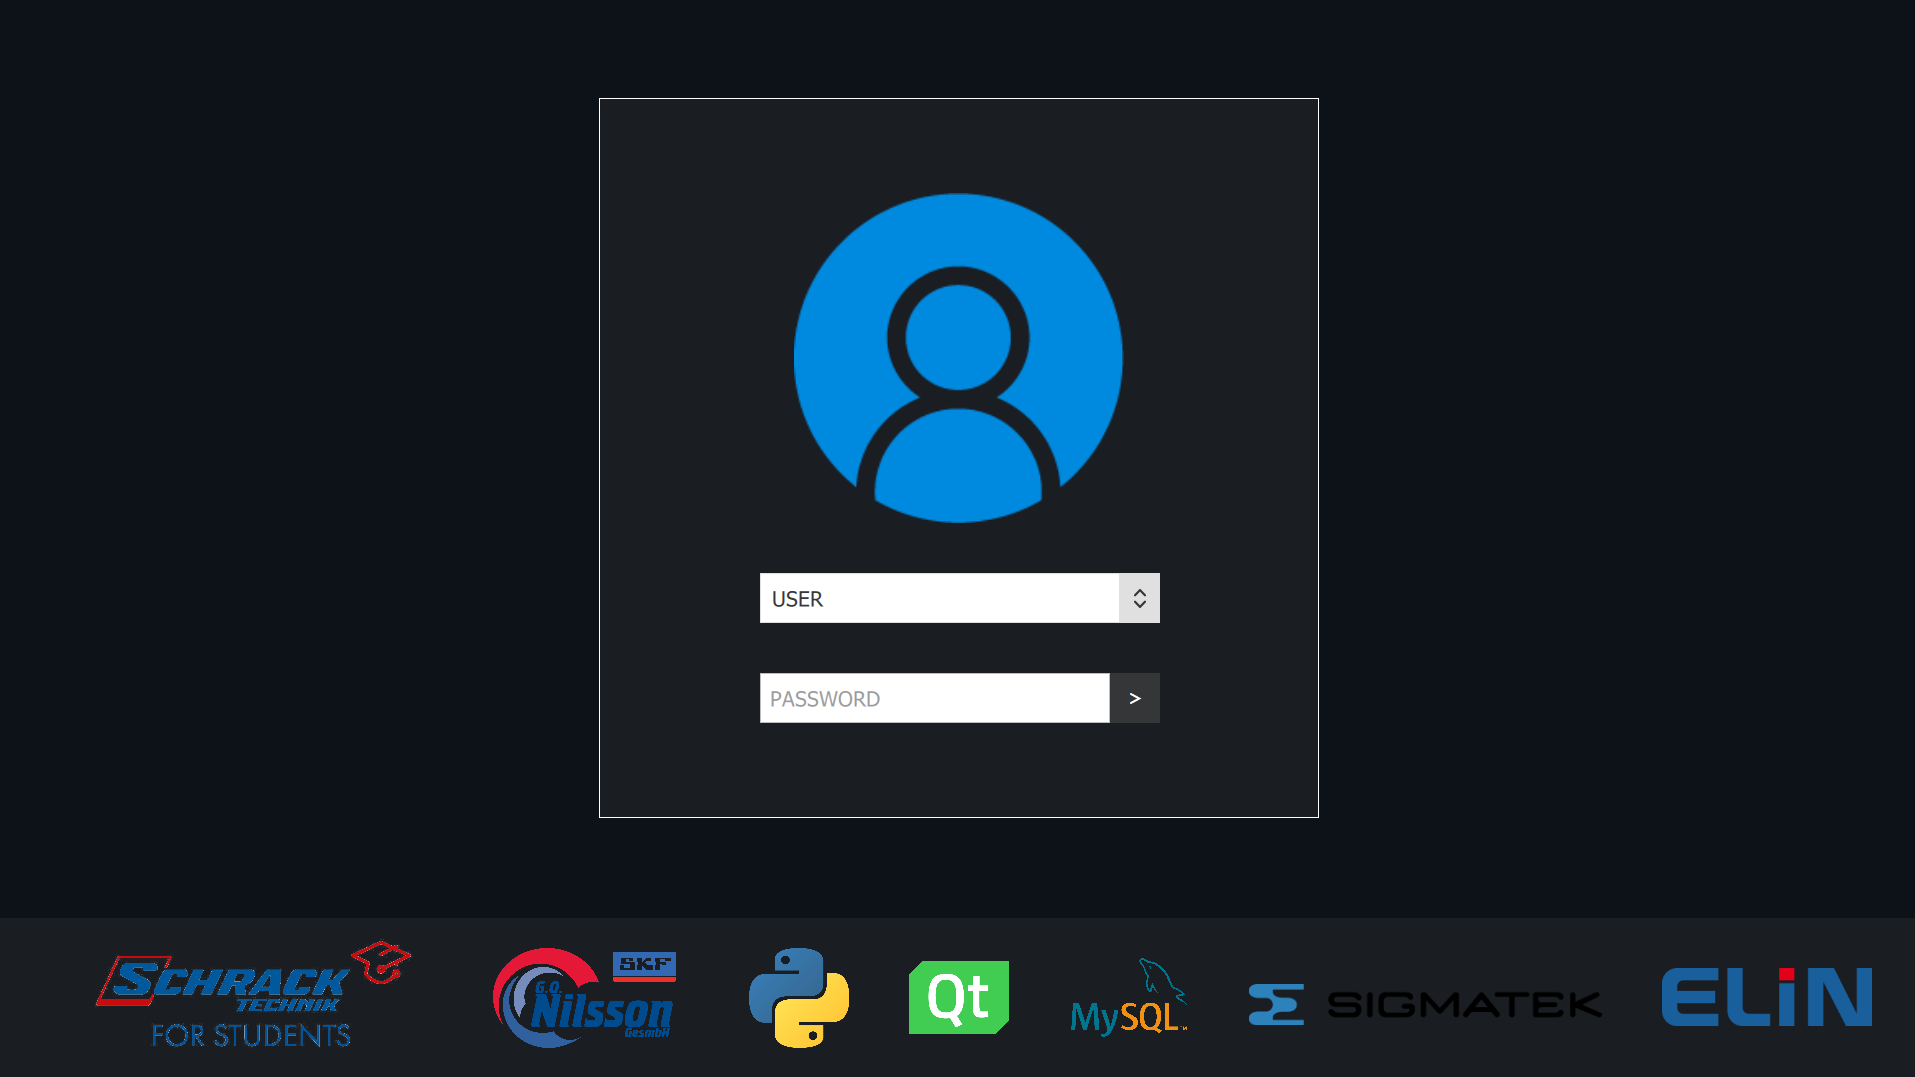
\includegraphics[scale=0.25]{figures/hcis/window_login.png}
			\caption{GUI Fenster - Login Menü}
			\label{fig:pageMenu}
	\end{center}
\end{figure}

 Um sich einzuloggen muss nur mehr das Passwort im \textit{Textfeld} darunter eingegeben werden. Nach dem Drücken des Login Pfeiles (Neben dem Passwort Textfeld) werden die Login Daten an das Backend versendet. Diese vergleicht die Daten über die Datenbankschnittstelle\footnote{siehe Abschnitt} und loggt, insofern das richtige Passwort gegeben ist, den Benutzer ein. Wird jedoch das Passwort falsch eingegeben, wird eine rote Fehlermeldung angezeigt.\\
 
\subsubsection{Fahrdaten}		

Dieses Fenster dient als Ersatz für die Instrumententafel des Motorrades. Es ist daher das einzige während der Fahrt ersichtliche Fenster. Es Zeigt alle wichtigen Fahrdaten wie Leistung, Geschwindigkeit und Akkuladestand, sowie den Aktuellen Fahrmodus an. Diese Anzeige kann jedem Nutzer, unabhängig der Berechtigung, angezeigt werden.

\begin{figure}[H]
	\begin{center}
		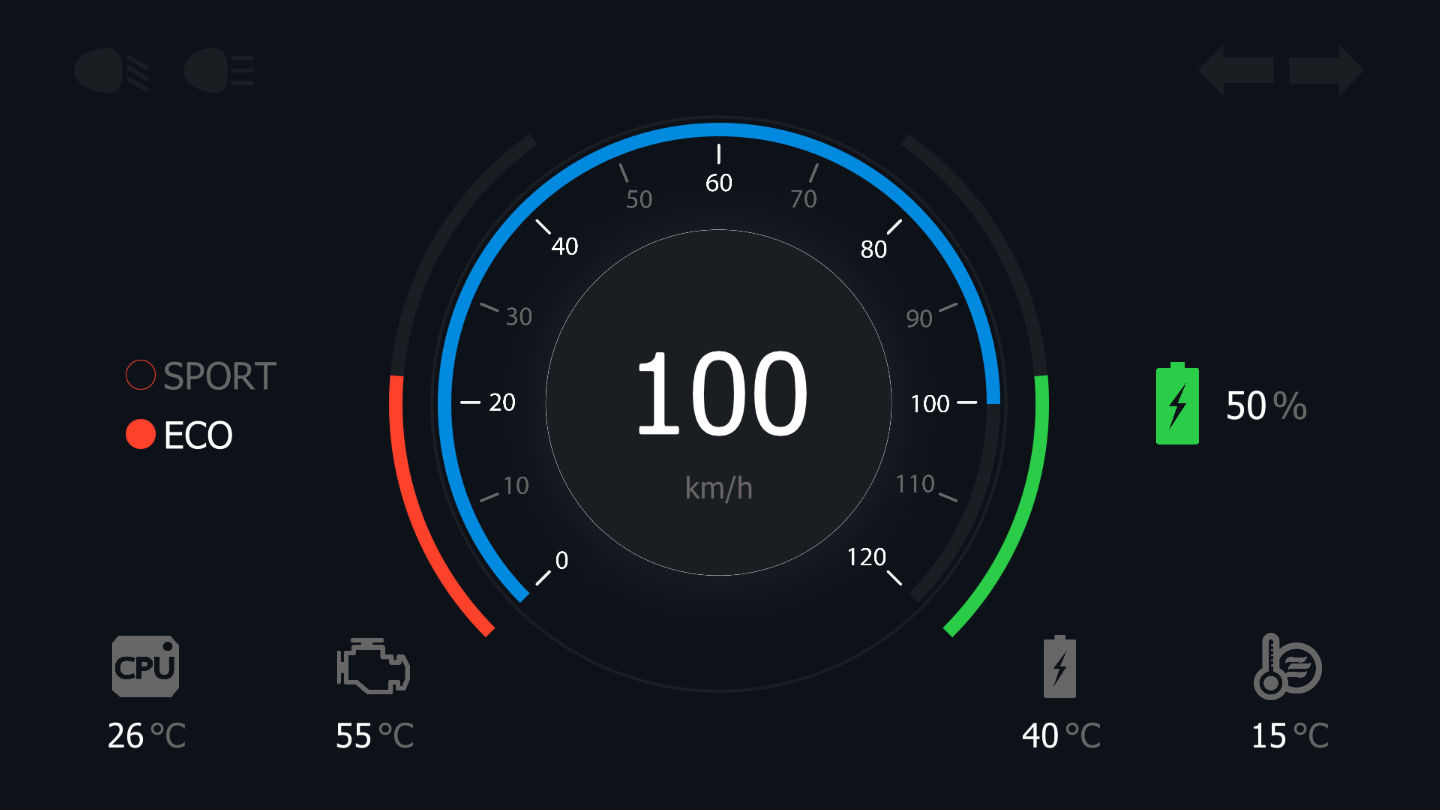
\includegraphics[scale=0.25]{figures/hcis/window_dashboard.png}
			\caption{GUI Fenster - Fahrdaten}
			\label{fig:pageDash}
	\end{center}
\end{figure}

Der Status der Blinker und der Beleuchtung wird ebenso wie die Temperaturen der verschiedenen Komponenten des Motorrades angezeigt. Derzeit ist diese Ansicht starr und kann noch nicht geändert werden. Doch es ist geplant in Zukunft weitere Designs, welche in den Einstellungen geändert werden können, zu implementieren.

\newpage

\subsubsection{Akku- und Ladedaten}

Dieses Fenster dient Ähnlich wie das der Fahrdaten zur Darstellung wichtiger Daten. Es können alle wichtigen Daten bezüglich Akku und BMS auf einem Blick abgelesen werden. 

\begin{figure}[H]
	\begin{center}
		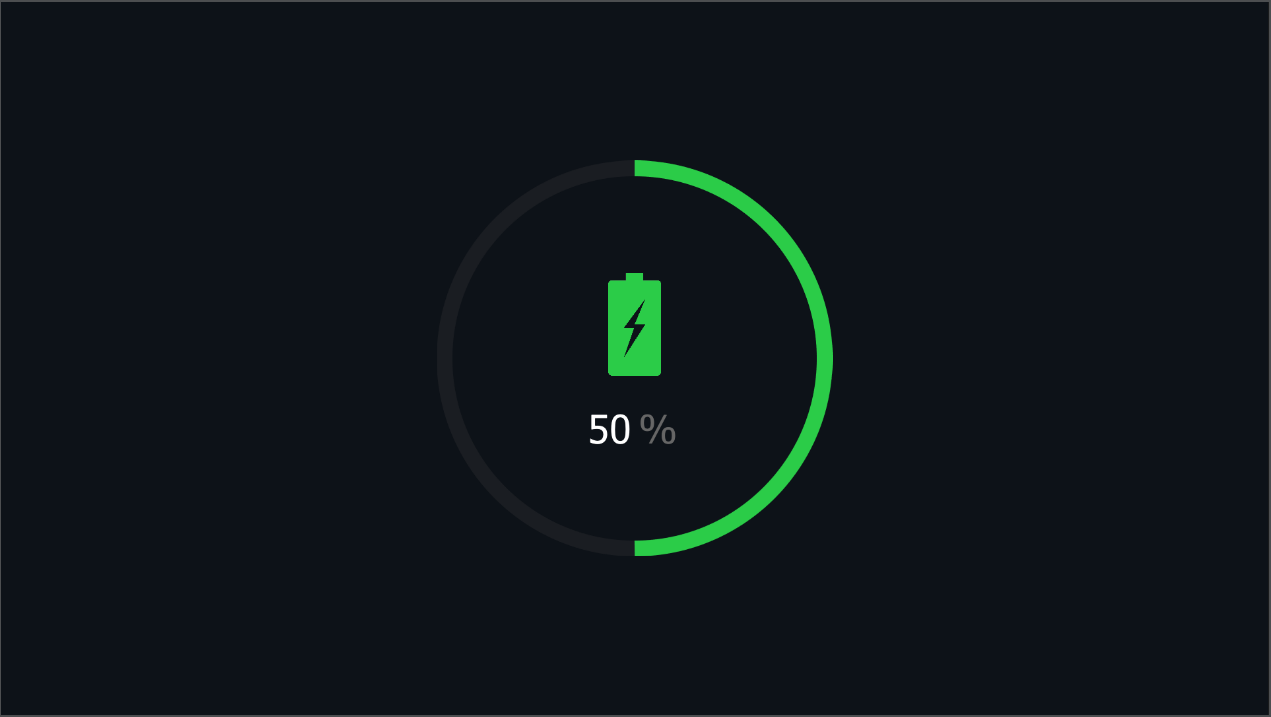
\includegraphics[scale=0.25]{figures/hcis/window_battery.png}
			\caption{GUI Fenster - Akkudaten}
			\label{fig:pageAkku}
	\end{center}
\end{figure}

Dieses Fenster wird Standardmäßig während dem Laden des Fahrzeuges angezeigt. Es benötigt also keine bestimmte Berechtigung und kann von jedem Nutzer über das Navigations-Menü angezeigt werden.

\subsubsection{Fahrdaten Diagnose}

Hier können die Fahrdaten, welche während der Fahrt dauerhaft von der Motorsteuerung versendet und vom Raspberry Pi verarbeitet und in einer Datenbank gespeichert werden, in Graphen angezeigt werden. Hierzu wird die \textit{Graph Komponente} \footnote{siehe Abschnitt \ref{sec:graph}} verwendet.
\begin{figure}[H]
	\begin{center}
		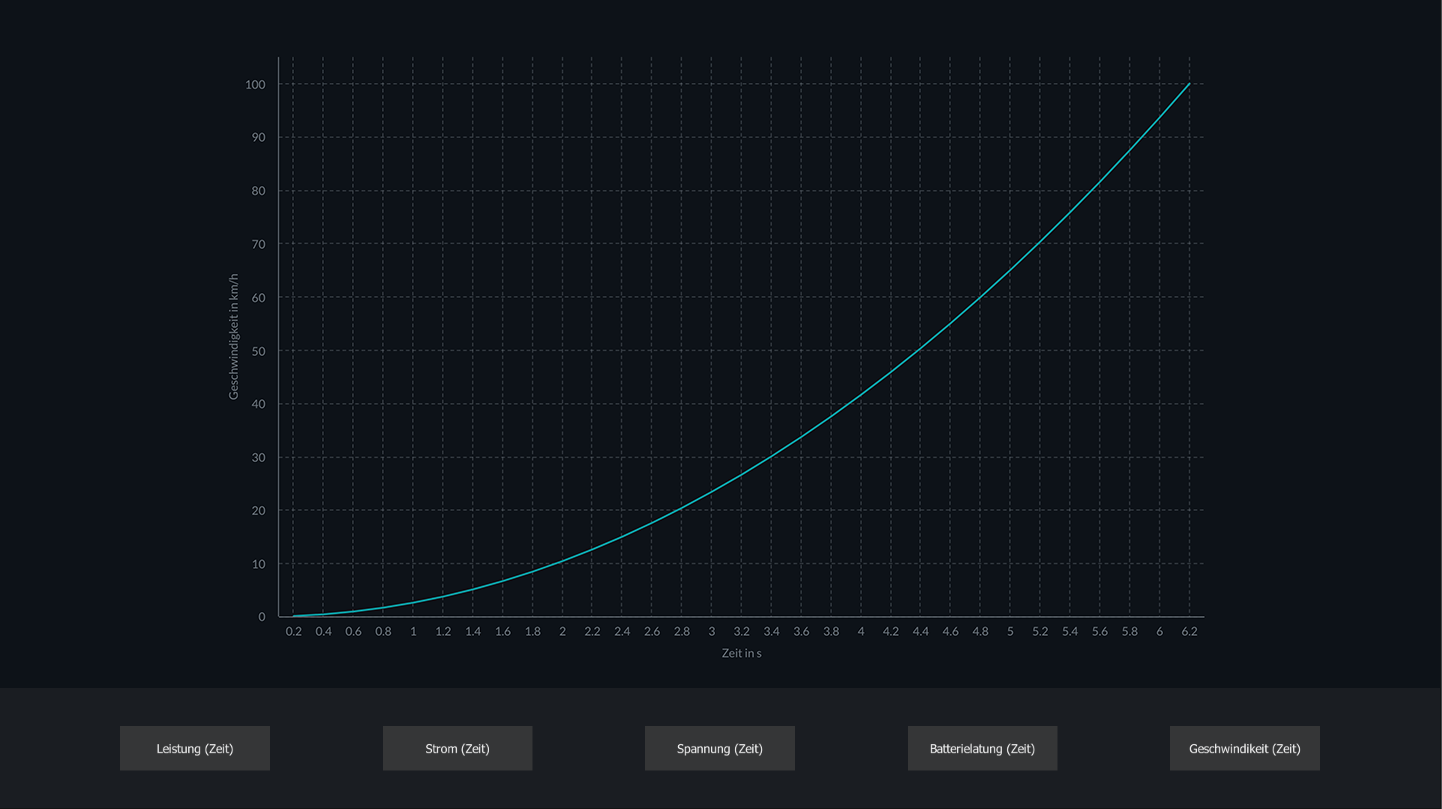
\includegraphics[scale=0.25]{figures/hcis/window_diagnosis.png}
			\caption{GUI Fenster - Fahrdaten Diagnose}
			\label{fig:pageDiagnose}
	\end{center}
\end{figure}

 Diese wird, um während der Fahrt die volle Prozessorleistung zu gewährleisten, erst auf Knopfdruck geladen. In der Menüleiste am unteren Ende des Fensters können verschiedene Vorlagen ausgewählt werden, welche über fixe Datensätze verfügen. Das bedeutet es werden erst beim Auswählen des anzuzeigenden Datensatzes die Daten der letzten Stunde ausgelesen und in den Graphen geladen.


\newpage

\subsubsection{Fehler}

Sobald ein Fehlerdatenpaket über den CAN-Bus versendet wird, gibt der Listener Klasse die Fehlercodes an die Bridge Klasse weiter, um sie in diesem Fenster anzuzeigen. In einer \textit{Listview} werden nun die Aktiven Fehler angezeigt. Solange Fehler anliegen werden diese angezeigt und erst sobald die zuvor angezeigten Fehler nicht mehr anliegen werden diese aus der Liste gelöscht.

\begin{figure}[H]
	\begin{center}
		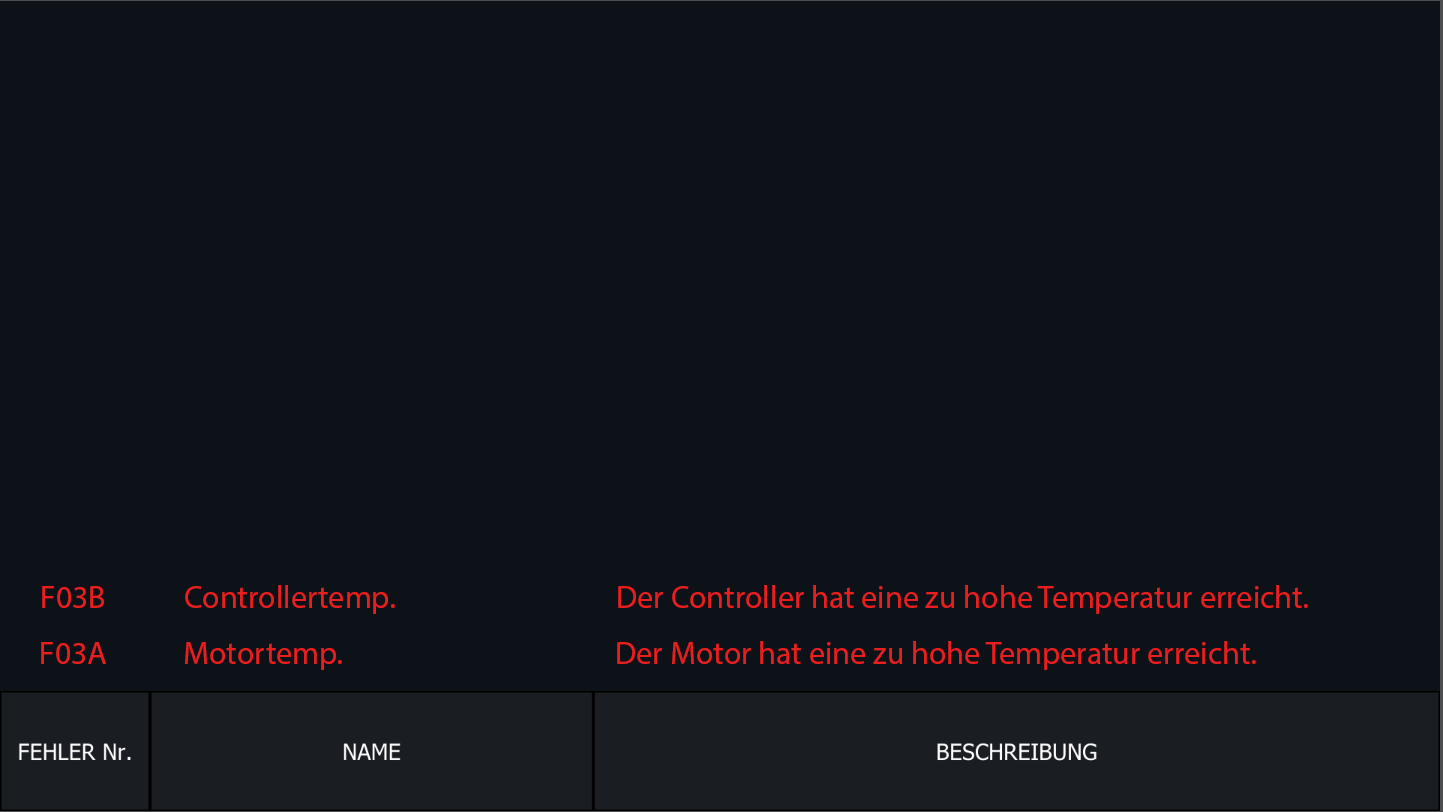
\includegraphics[scale=0.25]{figures/hcis/window_error.png}
			\caption{GUI Fenster - Fehler Liste}
			\label{fig:pageError}
	\end{center}
\end{figure}

Der Name und die Beschreibung der Fehler, wird über eine Fehlertabelle\footnote{siehe Abschnitt } in der Datenbank ausgelesen. Diese werden während dem Testen des Motorrades gesammelt und häufig auftretende Fehler werden in diese Tabelle eingetragen. 

\subsubsection{Nutzer und Berechtigungen}

Um sicherzustellen das das Nutzen der Benutzeroberfläche nicht für jeden uneingeschränkt möglich ist wurde ein Anmeldesystem mit drei verschiedenen Benutzern, welche jeweils verschiedene Berechtigungen besitzen, umgesetzt.

{\small \textbf{ADMIN}} - Passwort: 53AC2\\ \vspace{2mm}


Dieser Benutzer verfügt über uneingeschränkte Rechte und kann auf jede verfügbare Funktion sowie Funktionen, welche noch in Entwicklung sind zugreifen.

{\small \textbf{USER}} - Passwort: 5AHET\\ \vspace{2mm}

Dieser Benutzer verfügt über wenig eingeschränkte Rechte. Er kann auf jede fertig entwickelte Funktion zugreifen kann jedoch keine Änderungen an der Benutzeroberfläche vornehmen und hat ebenso keinen Zugriff auf experimentelle Funktionen.

{\small \textbf{GUEST}} - Passwort: 00000\\ \vspace{2mm}

Dieser Benutzer verfügt nur über sehr eingeschränkte Rechte. Er wird zum Präsentieren der Maschine benützt und lässt den unerfahrenen Nutzer nur auf die Fahrdaten und Akku- und Ladedaten zugreifen. Ebenso sollte in Zukunft die Leistung des Motorrades beim einloggen dieses Benutzers stark eingeschränkt werden, um Unfälle zu verhindern.

\newpage

\subsection{Realisierung der Benutzeroberfächer}

\subsubsection{QML} \label{sec:qml}
QML \footnote{Qt Modeling Language} ist eine deklarative Sprache, mit der Benutzeroberflächen anhand ihrer visuellen Komponenten und ihrer Interaktion und Beziehung zueinander beschrieben werden können. Es ist eine gut lesbare Sprache, die entwickelt wurde, um die dynamische Verbindung von Komponenten zu ermöglichen und die die einfache Wiederverwendung und Anpassung von Komponenten innerhalb einer Benutzeroberfläche erlaubt. Es bietet  Syntax mit Unterstützung für Java-Script-Ausdrücke in Kombination mit dynamischen Eigenschaftsverbindungen.

\subsubsection{Qt-Quick}
Das Qt-Quick-Modul ist die Standardbibliothek zum schreiben von QML-Anwendungen. Während das QML-Modul die Engine und die Sprachinfrastruktur bereitstellt, bietet das Qt Quick-Modul alle grundlegenden Typen, die zum Erstellen von Benutzeroberflächen mit QML erforderlich sind. Es bietet eine visuelle Zeichenfläche und Typen zum Erstellen und Animieren visueller Komponenten, zum Empfangen von Benutzereingaben, zum Erstellen von Datenmodellen und Ansichten sowie zum verzögerten Objektinstanziieren. Es können problemlos flüssige, animierte Benutzeroberflächen in QML erstellt werden. Diese Benutzeroberflächen können mit beliebigen Backend Bibliotheken verbunden werden.

\subsubsection{Slots und Signals} \label{sec:slots}
Slots und Signals werden in QML zur ereignisgesteuerten Kommunikation zwischen Frontend und Backend verwendet. In der folgenden Illustration wird diese anhand eines einfachen Beispiels erklärt.

\begin{figure}[H]
	\begin{center}
		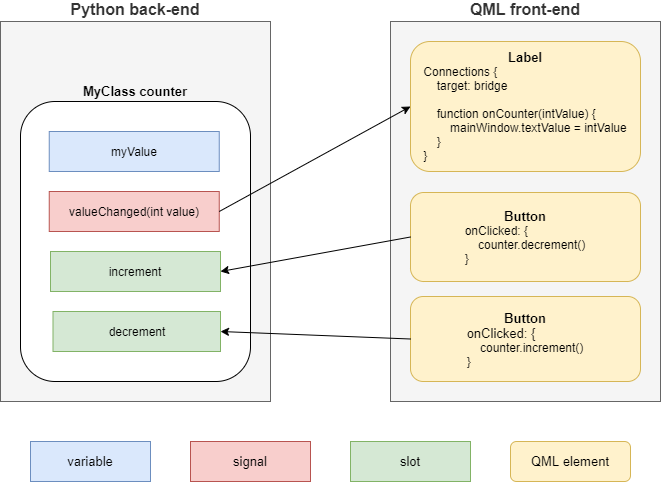
\includegraphics[scale=0.4]{figures/hcis/signals_slots.png}
		\caption{Slots und Signals Konzept}
	\end{center}
\end{figure}

\textbf{Signale}\\ \medskip
Diese können als Mitteilungen angesehen werden, welche über das Aufrufen der \textit{signal.emit()} Funktion vom Backend an das Frontend gesendet wird. Im Frontend wird wiederum eine eigens definierte Funktion benötigt um dem Wert einem Property eines QML Elements zuzuweisen.
\medskip

\textbf{Slots}\\ \medskip
Slots sind Call-Back Funktionen, welche im Backend definiert werden und sind über die Bridge Klasse mit dem Frontend verknüpft. Dadurch können diese Funktionen im Frontend aufgerufen und mit Signalen verbunden werden. Sie stellen daher die wichtigste Verbindung zwischen dem Programm und der Benutzeroberfläche dar.

\newpage
	
\subsubsection{Bridge}

Die Bridge Klasse wird für die Kommunikation zwischen den einzelnen Module des Backends mit denen der graphischen Benutzeroberfläche. 

\begin{figure}[H]
	\begin{center}
		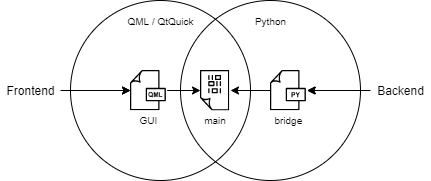
\includegraphics[scale=0.33]{figures/hcis/bridge.png}
		\caption{Verbindung Frontend zu Backend}
	\end{center}
\end{figure}

\newpage

%% Kommunikation %%%%%%%%%%%%%%%%%%%%%%%%%%%%%%%%%%%%%%%%%%%%

\section{Kommunikation}

Um Daten zwischen den mehreren Steuereinheiten des Motorrades zu versenden, muss eine Echtzeit-Kommunikation über ein Bussystem gewährleistet werden. Die Entscheidung ist auf das Controller Area Network Bussystem (CAN-Bus) gefallen. Ausschlaggebend für diese Entscheidung war der Curtis Motorcontroller, dieser verfügt über eine serielle Schnittstelle (RS-232) sowie ein CAN-System. Für unserer Anwendung bietet das CAN-System eine größere Ausbaufähigkeit sowie größere Übertragungsraten, weshalb wir uns letztendlich auch dafür entschieden haben.

\subsection{Hardware}

\subsubsection{CAN-Modul}

Da der Raspberry Pi selbst nicht über ein CAN-System verfügt, erfolgt der Anschluss an die Busleitung über ein externes CAN-Modul, welches über das Serial Peripheral Interface (SPI) mit dem Raspberry Pi kommuniziert, welches wie folgt angeschlossen werden muss: 

\begin{figure}[H]
	\begin{center}
		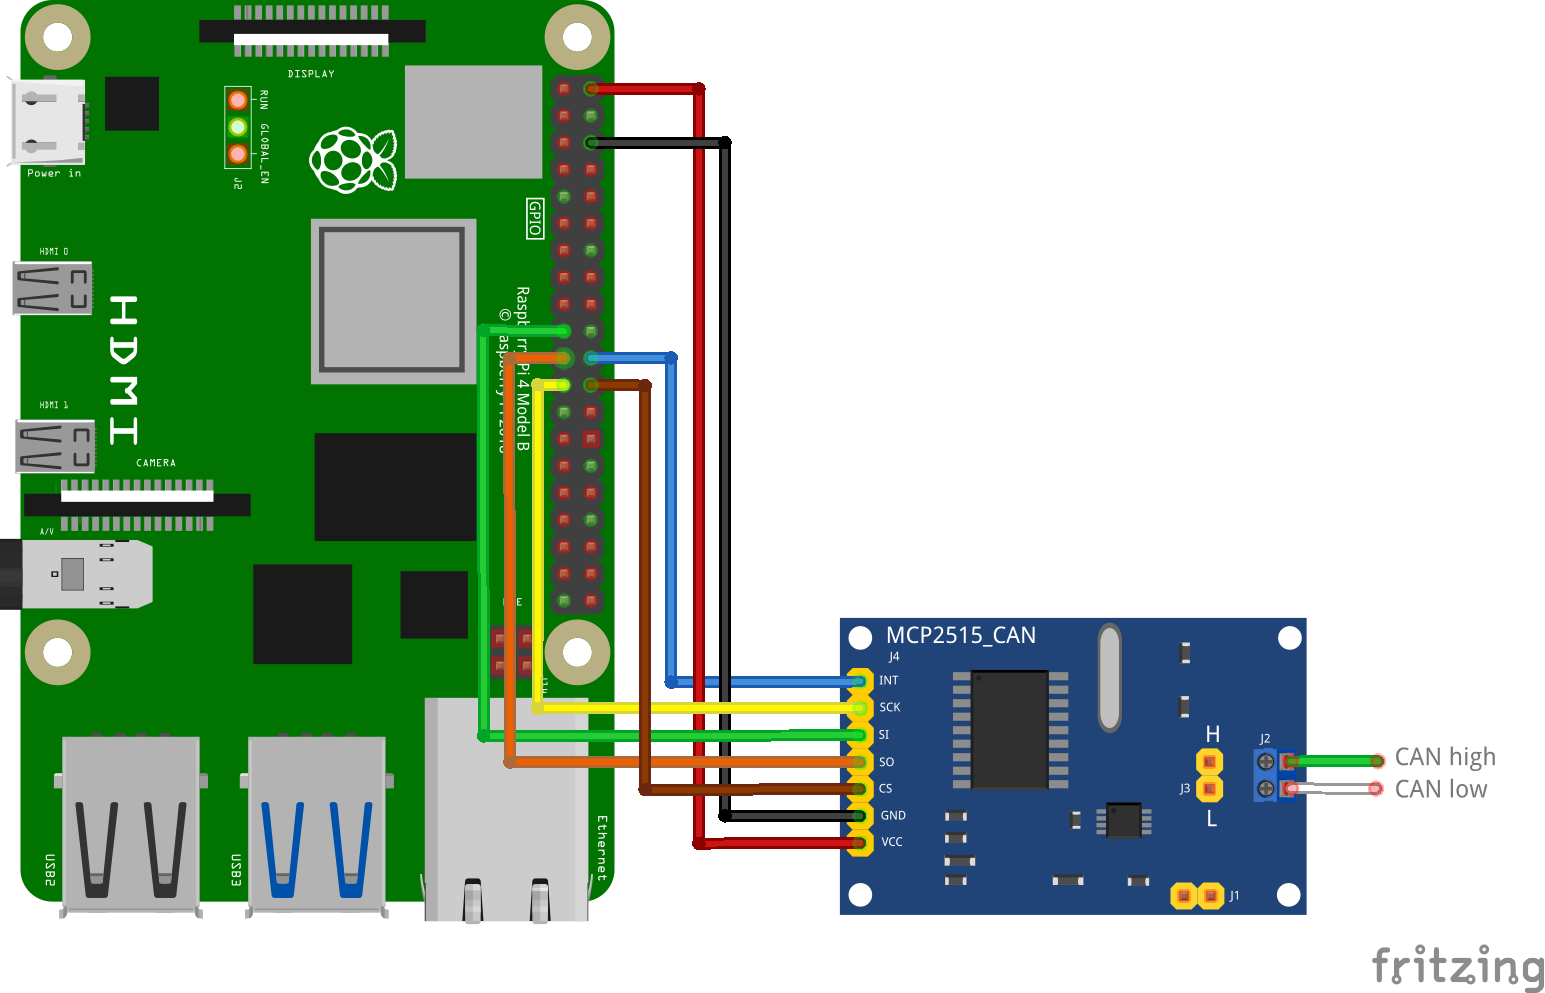
\includegraphics[scale=0.9]{figures/hcis/can_module.png}
		\caption{Anschlussplan CAN-Modul}
	\end{center}
\end{figure}

Die Kommunikation wird über zwei Komponenten ermöglicht. Einen MCP2562 Transceiver, welcher für die Verarbeitung der Nachrichten zuständig ist und ein MCP2515 CAN Interface, welches die Daten zwischenspeichert und sich um das Versenden der Nachrichten kümmert. Gemeinsam mit dem Mikrocomputer ergibt dies nun einen CAN Node, welcher fähig ist Nachrichten zu versenden und zu empfangen.

\subsubsection{Netzwerkstruktur}

Ein CAN-Netzwerk wird standardmäßig als Bus- oder Sterntopologie aufgebaut. Wir haben uns bewusst für die Bustopologie entschieden, da Sterntopologien nur in bestimmten Anwendungen Gebrauch finden und noch dazu markante Nachteile besitzt.\\ Es müsste zum Beispiel eine zentrale Steuereinheit den Nachrichtenverkehr steuern, ebenso gibt uns die niedrige Anzahl an Teilnehmern im Netzwerk nicht einmal die Möglichkeit ein anderes System zu verwenden. Erst wenn wir in Zukunft das CAN-Netzwerk um Sensoren und Aktoren erweitern würden, müsste weitere Zeit in die Planung des Netzwerks investiert werden. 

\newpage

\subsection{Listener}

Die Listener Klasse ist dafür zuständig den Datenverkehr am Bus zu überwachen und geordnet an die Datenbankschnittstelle \footnote{siehe Abschnitt} sowie die Schnittstelle zum Frontend (Bridge) weiterzugeben.

\subsubsection{Konfigurieren der Schnittstelle}
	
\begin{lstlisting}[language=Python, caption={Konfigurieren des CAN Adapters},captionpos=b]
	

	
\end{lstlisting}

\subsubsection{Empfangen der Daten}



\newpage

%% Fahrdatenspeicher %%%%%%%%%%%%%%%%%%%%%%%%%%%%%%%%%%%%%%%%

\section{Fahrdatenspeicher}

Das Motorrad sollte seine Fahrdaten abspeichern und darstellen können, um eine Diagnose des gesamten Aufbaus zu gewährleisten. Dafür wird eine Datenbank verwendet, nämlich die weit verbreitete Software MySQL verwendet.

\subsection{Datenbankstruktur}

\subsubsection{Benutzer System}

id ist nicht signiert und ist der Primärschlüssel mit Auto-Inkrement.

\begin{table}[H]
	\begin{center}
		\begin{tabular}{|c|c|l|}
		\hline
		\multicolumn{3}{|c|}{\textbf{users}}                          \\ \hline
		\textbf{Attribut} & \textbf{Datentyp} & \textbf{Beschreibung} \\ \hline
		id                & int               & Identifikationsnummer \\ \hline
		username          & varchar(50)       & Name des Benutzers    \\ \hline
		password          & varchar(255)      & Eingegebenes Passwort \\ \hline
		\end{tabular}
		\caption{Datenbankstruktur der Benutzer Tabelle}
		\label{tab:logindata}
	\end{center}
\end{table}

\subsubsection{Motor Daten}

\textbf{Datenpacket 1}
 
\begin{table}[H]
	\begin{center}
		\begin{tabular}{|c|c|l|}
			\hline
			\multicolumn{3}{|c|}{\textbf{data1}} \\ \hline
			\textbf{Attribut} & \textbf{Datentyp} & \textbf{Beschreibung}            \\ \hline
			id                & int               & Identifikationsnummer            \\ \hline
			date\_time        & datetime          & Datum der Erstellung             \\ \hline
			vehicle\_speed    & int               & Geschwindigkeit des Motorrades   \\ \hline
			current\_rms      & int               & Ausgangsstrom der Motorsteuerung \\ \hline
			controller\_temp  & int               & Temperatur des Kontrollers       \\ \hline
			motor\_temp       & int               & Temperatur des Motors            \\ \hline
			motor\_torque     & int               & Drehmoment am Motor              \\ \hline
			modulation\_depth & int               & Modulationsgrad des Kontrollers  \\ \hline
		\end{tabular}
			\caption{Datenbankstruktur der Datenpaket 1 Tabelle}
			\label{tab:data1}
	\end{center}
\end{table}

id ist nicht signiert und ist der Primärschlüssel mit Auto-Inkrement.
step id ist ein Z¨ahlerattribut, das f ¨ ur die Reihenfolge der Schritte verwendet wird, wie
sie in der grafischen Oberfl¨ache angezeigt werden. Der kaskadierte Fremdschl ¨ ussel
tutorial id wird f ¨ ur die Zuordnung zu dem jeweiligen Tutorial verwendet. F¨ ur die

\newpage

\textbf{Datenpacket 2}

\begin{table}[H]
	\begin{center}
		\begin{tabular}{|c|c|l|}
			\hline
			\multicolumn{3}{|c|}{\textbf{data2}} \\ \hline
			\textbf{Attribut}  & \textbf{Datentyp} & \textbf{Beschreibung}               \\ \hline
			id                 & int               & Identifikationsnummer               \\ \hline
			id\_data\_1        & int               & Fremdschlüssel von Datenpaket 1     \\ \hline
			date\_time         & datetime          & Datum der Erstellung                \\ \hline
			vehicle\_speed     & int               & Geschwindigkeit des Motorrades      \\ \hline
			capacitator\_volts & int               & Eingangsspannung der Motorsteuerung \\ \hline
			bdi\_percentage    & int               & Ladestand des Akkus              	 \\ \hline
			interlock          & int               & Muss aktiv sein um zu fahren        \\ \hline
			throttle\_command  & int               & Stellung des Gasgriffes             \\ \hline
			brake\_command     & int               & Stellung der Motorbremse (software) \\ \hline
			driving\_mode      & int               & Aktueller Fahrmodus                 \\ \hline
		\end{tabular}
			\caption{Datenbankstruktur der Datenpaket 2 Tabelle}
			\label{tab:data2}
	\end{center}
\end{table}

\textbf{Datenpacket 3}

\begin{table}[H]
	\begin{center}
		\begin{tabular}{|c|c|l|}
			\hline
			\multicolumn{3}{|c|}{\textbf{data3}} \\ \hline
			\textbf{Attribut}           & \textbf{Datentyp} & \textbf{Beschreibung}                     	\\ \hline
			id                          & int               & Identifikationsnummer                     	\\ \hline
			id\_data\_2                 & int               & Fremdschlüssel von Datenpaket 2          		\\ \hline
			date\_time                  & datetime          & Datum der Erstellung                      	\\ \hline
			vehicle\_speed              & int               & Geschwindigkeit des Motorrades            	\\ \hline
			vehicle\_accelration        & int               & Eingangsspannung der Motorsteuerung       	\\ \hline
			vehicle\_odometer           & int               & Vom Motorrad zurückgelegte Strecke        	\\ \hline
			time\_to\_capture\_speed    & int               & Zeit bis zur eingestellten Geschwindigkeit 	\\ \hline
			time\_to\_capture\_distance & int               & Zeit bis zur eingestellten Distanz        	\\ \hline
			braking\_distance\_captured & int               & Zeit von Bremsbeginn bis zu Stillstand     	\\ \hline
			distance\_since\_stop       & int               & Zurückgelegte Distanz seit dem Stillstand	 	\\ \hline
		\end{tabular}
		\caption{Datenbankstruktur der Datenpaket 3 Tabelle}
		\label{tab:data3}
	\end{center}
\end{table}

\newpage

\textbf{Datenpacket 4 - Fehler}

\begin{table}[H]
	\begin{center}
		\begin{tabular}{|c|c|l|}
			\hline
			\multicolumn{3}{|c|}{\textbf{data4}} \\ \hline
			\textbf{Attribut}           & \textbf{Datentyp} & \textbf{Beschreibung}                     \\ \hline
			id                          & int               & Identifikationsnummer                     \\ \hline
			id\_data\_3                 & int               & Fremdschlüssel von Datenpacket 3          \\ \hline
			date\_time                	& datetime          & Datum der Erstellung        				\\ \hline
			error\_1                 	& int	            & Fehlercode 1                      		\\ \hline
			error\_2            		& int               & Fehlercode 2            					\\ \hline
			error\_3        			& int               & Fehlercode 3       						\\ \hline
			error\_4           			& int               & Fehlercode 4       	 					\\ \hline
			error\_5    				& int               & Fehlercode 5 								\\ \hline
			error\_6					& int               & Fehlercode 6        						\\ \hline
			error\_7					& int               & Fehlercode 7    							\\ \hline
		\end{tabular}
		\caption{Datenbankstruktur der Fehler-Datenpaket Tabelle}
		\label{tab:data4}
	\end{center}
\end{table}

\subsubsection{Fehler Tabelle}

Diese Tabelle ist ebenso in der Datenbank gespeichert. Sie beinhaltet die Fehlercodes der Motorsteuerung mit weiteren Informationen wie Name und Beschreibung. Sie muss per Hand angelegt werden und sollte während dem Testen der Maschine mit dokumentiert, um sie dann in das Fehler Fenster der Benutzeroberfläche zu implementieren.

\subsubsection{Akku Daten}

Da die Kommunikation der BMS noch nicht umgesetzt wurde, werden von Ihr keine Daten auf den CAN-Bus gelegt und daher muss auch keine Tabelle dafür erstellt werden. Somit werden alle Daten über Akku und Ladestand über die Motorsteuerung empfangen.

\subsection{Handler}

Die Handler Klasse hat die Aufgabe eine Verbindung zwischen der Datenbank und dem Programm herzustellen. Dazu verwendet sie die MySQL-Connector Bibliothek. Mit dieser können SQL Skripten direkt in die Python Klasse integriert werden ohne dass externe SQL Skript Dateien geöffnet werden müssen.

Dieser bekommt in Echtzeit eine Liste der aktuell Empfangenen Daten der Listener Klasse \footnote{siehe Abschnitt } und schreibt diese in die dafür vorgesehenen Tabelle der Datenbank. Hierfür wird ein eigener Thread \footnote{siehe Abschnitt } geöffnet, um diese Aufgabe unabhängig von dem Restlichen Programm ausführen zu können.

Ebenso verfügt er über Funktionen, welche über das Diagnose Fenster \footnote{siehe Abschnitt } angewählt werden können und Daten aus der Datenbank auslesen, um sie in einem Graph anzeigen zu lassen.

\subsubsection{Konfigurieren der Schnittstelle}

Um auf eine Datenbank zu zugreifen wird muss ein \textit{connect} Objekt, mit den Anmeldedaten der lokalen Datenbank als Parameter, erstellt werden. Mit diesem Objekt kann nun auf Subklassen zugegriffen werden und Daten können aus- und eingelesen werden.

\begin{lstlisting}[language=Python, caption={Konfiguration der Datenbankschnittstelle},captionpos=b]
	
	# Database credentials
	dbhost = "hostname"
	dbuser = "username"
	dbpass = "password"
	dbname = "databasename"
	
	# Connection to the database
	con = mysql.connector.connect(host=dbhost, user=dbuser, password=dbpass, database=dbname)
	
\end{lstlisting}

\newpage

\subsubsection{Cursor klasse}

Die Cursor Klasse instanziiert Objekte, die Operationen wie SQL-Anweisungen ausführen können. Cursor interagieren mit dem Server mithilfe eines Connection Objekts. Sie können 

\begin{lstlisting}[language=Python, caption={Erstellen eines Cusorobjekts},captionpos=b]
	
	# Creating cursor for database queries
	cursor = con.cursor()
	
\end{lstlisting}

Einpaar der Wichtigsten Befehle sind:

\begin{itemize}
	
	\item \textit{cursor.execute()} \\ Diese Methode führt die angegebene Abfrage aus. Die in den Tupel- oder Wörterbuchparametern gefundenen Parameter sind an die Variablen in der Operation gebunden. Geben Sie Variablen mit dem Parameterstil von \% s oder \% (Name) an.
	
	\item \textit{cursor.fetchall()} \\ Diese Methode ruft alle Zeilen einer Abfrage ab und gibt eine Liste von Tupeln \footnote{ein Datensatz (eine Zeile) einer Datenbank} zurück. Wenn keine Zeilen mehr verfügbar sind, wird eine leere Liste zurückgegeben.
	
	\item \textit{cursor.close()} \\ Diese Methode wird verwendet wenn man einem Cursor nicht mehr benötigt. Diese Methode schließt den Cursor, setzt alle Ergebnisse zurück und stellt sicher, dass das Cursorobjekt keinen Verweis auf sein ursprüngliches Verbindungsobjekt hat.
	
\end{itemize}

\subsubsection{SELECT Befehl}

Der SELECT Befehl wird zum Abrufen von Daten einer Tabelle verwendet und besitzt mehrere Parameter.

\begin{lstlisting}[language=Python, caption={SELECT Befehl über MySQL Connector},captionpos=b]
		
	# Querying the data from the database
	sql = "SELECT * from users WHERE username = %s and password = %s"
	cursor.execute(sql, [(username), (password)])
	results = cursor.fetchall()
	
\end{lstlisting}

Der Befehl kann in zwei Bereiche unterteilt werden. In der ersten Zeile werden die
Attribute, die von der Tabelle ausgegeben werden sollen, definiert.  Die anzuzeigenden Ergebnisse werden durch den \textit{WHERE} Befehl gefiltert werden.
\\ Nützlich ist auch der Befehl JOIN durch den Tabellen anhand der Fremdschlüssel verbunden werden.

\subsubsection{INSERT Befehl}

Der INSERT Befehl wird zum Schreiben von Daten in eine Tabelle verwendet.

\begin{lstlisting}[language=Python, caption={INSERT Befehl über MySQL Connector},captionpos=b]
	
	# Inserting data into the database
	sql = "INSERT INTO `users` (`id`, `username`, `password`); VALUES (1, %s, %s);"
	cursor.execute(sql, [(username), (password)])
	
\end{lstlisting}

Dieser Befehl kann in zwei Teile unterteilt werden. In der ersten Zeile wird die Zieltabelle mit den Attributen angegeben. In der zweiten Zeile folgen die Werte, die in der Datenbank erfasst werden sollen. Hierbei ist die Reihenfolge der Attribute zu beachten. Das Attribut id wird standardmäßig von dem Datenbanksystem vergeben, es ist daher möglich das Attribut im Befehl zu vernachlässigen. \\
Als Wert wird ebenso die Funktion \textit{NOW()} unterstützt, wodurch intern der aktuelle Zeitstempel abgespeichert wird. Dadurch kümmert sich das Datenbanksystem um die korrekten Werte für das date\_time Attribut\footnote{siehe Abschnitt }.

\newpage